\documentclass[12pt, oneside]{book}
\usepackage[a4paper,top=2.5cm,bottom=2.5cm,left=3.5cm,right=2cm]{geometry}


\ifx\uv\undefined\newcommand{\uv}[1]{,,#1``}\fi  

\renewcommand{\baselinestretch}{1.5}  % pre zvascenie riadkovania
\let\openright=\clearpage

%%%%% Nastavení kódování vstupních souborů: UTF-8
%%%%% ---------------------------------------------------------------
\usepackage[utf8]{inputenc} 
\usepackage[slovak,english]{babel}
\usepackage[T1]{fontenc}
\usepackage{lmodern}
\usepackage{minted}
\usepackage[babel=true]{microtype}
\usepackage{siunitx}

\usemintedstyle{tango}
\usepackage{lastpage}
\usepackage{lmodern}
\usepackage{amsmath}
\usepackage{amssymb,amsfonts,amscd}
\usepackage{array,hhline}
\usepackage{makeidx}
\usepackage{graphicx}
\usepackage{listings}
\usepackage{xcolor}
\usepackage{eurosym}
\usepackage{psfrag}
\usepackage{caption}
\usepackage{makecell}
\usepackage{graphicx}
\usepackage{subfig}

%%% shadows
\usepackage{tikz}
\usetikzlibrary{shadows,calc}

% code adapted from https://tex.stackexchange.com/a/11483/3954

% some parameters for customization
\def\shadowshift{3pt,-3pt}
\def\shadowradius{6pt}

\colorlet{innercolor}{black!60}
\colorlet{outercolor}{gray!05}

% this draws a shadow under a rectangle node
\newcommand\drawshadow[1]{
    \begin{pgfonlayer}{shadow}
        \shade[outercolor,inner color=innercolor,outer color=outercolor] ($(#1.south west)+(\shadowshift)+(\shadowradius/2,\shadowradius/2)$) circle (\shadowradius);
        \shade[outercolor,inner color=innercolor,outer color=outercolor] ($(#1.north west)+(\shadowshift)+(\shadowradius/2,-\shadowradius/2)$) circle (\shadowradius);
        \shade[outercolor,inner color=innercolor,outer color=outercolor] ($(#1.south east)+(\shadowshift)+(-\shadowradius/2,\shadowradius/2)$) circle (\shadowradius);
        \shade[outercolor,inner color=innercolor,outer color=outercolor] ($(#1.north east)+(\shadowshift)+(-\shadowradius/2,-\shadowradius/2)$) circle (\shadowradius);
        \shade[top color=innercolor,bottom color=outercolor] ($(#1.south west)+(\shadowshift)+(\shadowradius/2,-\shadowradius/2)$) rectangle ($(#1.south east)+(\shadowshift)+(-\shadowradius/2,\shadowradius/2)$);
        \shade[left color=innercolor,right color=outercolor] ($(#1.south east)+(\shadowshift)+(-\shadowradius/2,\shadowradius/2)$) rectangle ($(#1.north east)+(\shadowshift)+(\shadowradius/2,-\shadowradius/2)$);
        \shade[bottom color=innercolor,top color=outercolor] ($(#1.north west)+(\shadowshift)+(\shadowradius/2,-\shadowradius/2)$) rectangle ($(#1.north east)+(\shadowshift)+(-\shadowradius/2,\shadowradius/2)$);
        \shade[outercolor,right color=innercolor,left color=outercolor] ($(#1.south west)+(\shadowshift)+(-\shadowradius/2,\shadowradius/2)$) rectangle ($(#1.north west)+(\shadowshift)+(\shadowradius/2,-\shadowradius/2)$);
        \filldraw ($(#1.south west)+(\shadowshift)+(\shadowradius/2,\shadowradius/2)$) rectangle ($(#1.north east)+(\shadowshift)-(\shadowradius/2,\shadowradius/2)$);
    \end{pgfonlayer}
}

% create a shadow layer, so that we don't need to worry about overdrawing other things
\pgfdeclarelayer{shadow} 
\pgfsetlayers{shadow,main}


\newcommand\shadowimage[2][]{%
\begin{tikzpicture}
\node[anchor=south west,inner sep=0] (image) at (0,0) {\includegraphics[#1]{#2}};
\drawshadow{image}
\end{tikzpicture}}

%%%

%%%%%% inline code
\definecolor{lightgray}{gray}{0.9}

\lstset{
    showstringspaces=false,
    basicstyle=\ttfamily,
    keywordstyle=\color{blue},
    commentstyle=\color[grey]{0.6},
    stringstyle=\color[RGB]{255,150,75}
}

\newcommand{\inlinecode}[1]{\colorbox{lightgray}{\lstinline[language=Bash]$#1$}}

%%%%%%

%%%%%%%%%%%%%%%%%%%%%%%%%%%%%%%%%%%%%%%%%%%%%%%%%%%%%%%%%%%%%%%%%%%%%%%%%%%%%%%%%%
%Define the listing package
\usepackage{listings} %code highlighter
\usepackage{color} %use color
\definecolor{mygreen}{rgb}{0,0.6,0}
\definecolor{mygray}{rgb}{0.5,0.5,0.5}
\definecolor{mymauve}{rgb}{0.58,0,0.82}
 
%Customize a bit the look
\lstset{ %
backgroundcolor=\color{white}, % choose the background color; you must add \usepackage{color} or \usepackage{xcolor}
basicstyle=\footnotesize, % the size of the fonts that are used for the code
breakatwhitespace=false, % sets if automatic breaks should only happen at whitespace
breaklines=true, % sets automatic line breaking
captionpos=b, % sets the caption-position to bottom
commentstyle=\color{mygreen}, % comment style
deletekeywords={...}, % if you want to delete keywords from the given language
escapeinside={\%*}{*)}, % if you want to add LaTeX within your code
extendedchars=true, % lets you use non-ASCII characters; for 8-bits encodings only, does not work with UTF-8
frame=single, % adds a frame around the code
keepspaces=true, % keeps spaces in text, useful for keeping indentation of code (possibly needs columns=flexible)
keywordstyle=\color{blue}, % keyword style
% language=Octave, % the language of the code
morekeywords={*,...}, % if you want to add more keywords to the set
numbers=left, % where to put the line-numbers; possible values are (none, left, right)
numbersep=5pt, % how far the line-numbers are from the code
numberstyle=\tiny\color{mygray}, % the style that is used for the line-numbers
rulecolor=\color{black}, % if not set, the frame-color may be changed on line-breaks within not-black text (e.g. comments (green here))
showspaces=false, % show spaces everywhere adding particular underscores; it overrides 'showstringspaces'
showstringspaces=false, % underline spaces within strings only
showtabs=false, % show tabs within strings adding particular underscores
stepnumber=1, % the step between two line-numbers. If it's 1, each line will be numbered
stringstyle=\color{mymauve}, % string literal style
tabsize=2, % sets default tabsize to 2 spaces
title=\lstname % show the filename of files included with \lstinputlisting; also try caption instead of title
}
%END of listing package%
 
\definecolor{darkgray}{rgb}{.4,.4,.4}
\definecolor{purple}{rgb}{0.65, 0.12, 0.82}
 
%define Javascript language
\lstdefinelanguage{JavaScript}{
keywords={typeof, new, true, false, catch, function, return, null, catch, switch, var, if, in, while, do, else, case, break},
keywordstyle=\color{blue}\bfseries,
ndkeywords={class, export, boolean, throw, implements, import, this},
ndkeywordstyle=\color{darkgray}\bfseries,
identifierstyle=\color{black},
sensitive=false,
comment=[l]{//},
morecomment=[s]{/*}{*/},
commentstyle=\color{purple}\ttfamily,
stringstyle=\color{red}\ttfamily,
morestring=[b]',
morestring=[b]"
}
 
\lstset{
language=JavaScript,
extendedchars=true,
basicstyle=\footnotesize\ttfamily,
showstringspaces=false,
showspaces=false,
numbers=left,
numberstyle=\footnotesize,
numbersep=9pt,
tabsize=2,
breaklines=true,
showtabs=false,
captionpos=b
}

%%%%%%%%%%%%%%%%%%%%%%%%%%%%%%%%%%%%%%%%%%%%%%%%%%%%%%%%%%%%%%%%%%%%%%%%%%%%%%%%%

\usepackage{url} 
\usepackage{bbding}         %%% balíček s nejrůznějšími
                            %%% symboly (čtverečky, hvězdičky,
                            %%% tužtičky, ručičky, nůžtičky, ...) 

\usepackage{paralist}       %%% lepší enumerate a itemize 
\usepackage{indentfirst}    %%% zaveď odsazení 1. odstavce
\usepackage[nottoc]{tocbibind} %%% zajistí přidání seznamu literatury,
                               %%% obrázků a tabulek do obsahu
\usepackage{tabularx}
\usepackage[pdftex,unicode,bookmarks=false]{hyperref}

\usepackage{fancyvrb}
\usepackage{fancyhdr} 
\fancyhf{}
\renewcommand{\headrulewidth}{0pt}
\cfoot{\thepage}

\usepackage{dirtytalk}
\usepackage{eurosym}

% \include{swift} % pridaný Swift highlighting

% Tato makra přesvědčují mírně ošklivým trikem LaTeX, aby hlavičky kapitol sázel příčetněji a nevynechával nad nimi spoustu místa. Směle ignorujte.
\makeatletter
\def\@makechapterhead#1{
  {\parindent \z@ \raggedright \normalfont
   \Huge\bfseries \thechapter. #1
   \par\nobreak
   \vskip 20\p@
}}
\def\@makeschapterhead#1{
 {\parindent \z@ \raggedright \normalfont
   \Huge\bfseries #1
   \par\nobreak
   \vskip 20\p@
}}
\makeatother

\newlength{\verbcorr}
\setlength{\verbcorr}{0ex}

\begin{document}

\selectlanguage{english}

\pagestyle{empty}
\pagenumbering{arabic}

%--------------------------------------------------------------------------------------
%%% hlavná stránka

\begin{titlepage}

\begin{center}

{\sc\LARGE University of Žilina}

\medskip

{\sc\Large Faculty of Management Science and Informatics}

\vfill\vfill\vfill\vfill

{\sc\LARGE Master's thesis}

\smallskip

{\large Field of study: {\bf Information systems}}

\end{center}

\vfill\vfill\vfill

\begin{center}
    
{\large\bf Jozef Chmelár}

\smallskip

{\large\bf Application of blockchain technology}

\smallskip

Tutor: {\bf Ing. Michal Kvet, PhD. }

\smallskip

Registration number : 760/2018	

\smallskip

ŽILINA 2019

\end{center}

\end{titlepage}

%--------------------------------------------------------------------------------------
%%% cestne vyhlásenie

\pagebreak
\hfill
\vfill

\begin{center}

\sc\Large\textbf{Declaration}

\end{center}

I hereby declare that this thesis was written by myself. I also declare that all the sources and information used  to complete the thesis are included in the list of references

\vspace{1em}

I agree with publication of this thesis.

\vspace{2em}

In Žilina, 2. May 2019    \hfill ...........................

\hfill Jozef Chmelár \hspace{0,5em}

% \vfill
% \hfill
\pagebreak

%--------------------------------------------------------------------------------------
%%% poďakovanie

\pagebreak
\hfill
\vfill

\begin{center}

\sc\Large\textbf{Acknowledgement}

\end{center}

I'd like to thank to my supervisor Ing. Michal Kvet, PhD . for his professional help, feedback and always pointing me to the right direction.

\vspace{2em}

In Žilina, 2. May 2019  \hfill ...........................

\hfill Jozef Chmelár \hspace{0,5em}

\pagebreak

%--------------------------------------------------------------------------------------
%%% slovensky abstrakt

\pagebreak

\begin{center}

\sc\Large\textbf{Abstrakt}
    
\end{center}

\noindent
{\sc CHMELÁR Jozef:} {\em Využitie technológie blockchain}
[Diplomová práca] 

\noindent
Žilinská univerzita v Žiline,  
Fakulta riadenia a informatiky,  
Katedra informatiky

\noindent  
Vedúci práce - Ing. Michal Kvet, PhD . Stupeň odbornej kvalifikácie - Inžinier.- Žilina: FRI ŽU v Žiline, 2018 - Počet strán \pageref{LastPage}
\noindent 



\vspace{1em}

Cieľom diplomvej práce je analýza technológie blockchain, jej použitie a súčasné implementácie. Vytvorenie aplikácie ktorá využíva blockchain na ukladanie výrobných dát. Tieto dáta musia byť uložené v nemennom stave aby poskytovali dôkaz o výrobe a zachovali integritu dát.

\vspace{1em}

\noindent
{\bf Kľúčové slová:} Blockchain, decentralizovaná databáza

\pagebreak

%--------------------------------------------------------------------------------------
%%% anglicky abstrakt

\selectlanguage{english}

\pagebreak

\begin{center}

\sc\Large\textbf{Abstract}
    
\end{center}

\noindent
{\sc CHMELÁR Jozef:} {\em Application of blockchain technology
}
[Master´s thesis] 

\noindent
University of Žilina,  
Faculty of Management Science and Informatics,  
Department of Informatics

\noindent  
Supervisor: Ing. Michal Kvet, PhD .  - Qualification level : Masters.- Žilina: FRI ŽU in Žilina ,2018 - Number of pages: \pageref{LastPage} 


\vspace{1em}

Thesis should analyze blockchain as a technology, its usage and current implementations. The goal is to develop a blockchain application for storing manufacturing data. This data should be stored in immutable state to provide proof of manufacturing and integrity of data.

\vspace{1em}

\noindent
{\bf Keywords:} Blockchain, decentralized database

\pagebreak

\selectlanguage{english}

\pagestyle{myheadings}

\setcounter{page}{7}

%%%%%%%%%%%%%%%%%% obsah

{
\setlength{\parskip}{1pt plus 1pt}

\markboth{}{}

\pagestyle{fancy}

% obsah
\tableofcontents

% zoznam obrazkov
\listoffigures

% zoznam tabuliek
\listoftables

% zoznam skratiek
\chapter*{List of Shortcuts}
\addcontentsline{toc}{chapter}{List of shortcuts}

\begin{tabularx}{\textwidth}{@{}>{\bfseries\raggedright\hsize=.4\hsize}X >{\hsize=1.6\hsize}X@{}}
        
    \textbf{P2P}  & Peer to peer                 \label{P2P}\\
    \textbf{MSP}  & Membership Service Providers \label{MSP}\\
    \textbf{PoET} & Proof of Elapsed Time        \label{MSP}\\
    \textbf{PoF}  & Proof of work                \label{MSP}\\
    \textbf{PoS}  & Proof of stake                \label{MSP}\\
    \textbf{PoC}  & Proof of capacity               \label{MSP}\\
    \textbf{CPU}  & Central processing unit      \label{MSP}\\
    \textbf{GPU}  & Graphics processing unit     \label{MSP}\\
    \textbf{AISC} & Application-specific integrated circuit         \label{MSP}\\
    \textbf{SHA}  & Secure hash algorithm        \label{MSP}\\
    \textbf{SGX}  & Software Guard Extensions    \label{MSP}\\
    \textbf{CRUD} & Create, read, update, delete   \label{MSP}\\
    \textbf{YAML} & YAML Ain't Markup Language   \label{MSP}\\
    \textbf{SDK}  & Sofware development kit                 \label{MSP}\\
    \textbf{API}  & Application programming interface        \label{MSP}\\
    \textbf{SQL}     & Structured Query Language                       \label{MSP}\\
    \textbf{NoSQL}     & Not only SQL                              \label{MSP}\\
    \textbf{REST}     & Representational state transfer                             \label{MSP}\\
    \textbf{PLC}  & Programmable logic controller                \label{MSP}\\
    \textbf{ASN.1}     & Abstract Syntax Notation One                               \label{MSP}\\
    \textbf{WPF}     & Windows presentation foundation                            \label{MSP}\\
    \textbf{HMI}     & Human machine interface                           \label{MSP}\\
    \textbf{POCO}     & Plain old CLR objects                             \label{MSP}\\

    \textbf{MVVM}     & Model-View-ViewModel                             \label{MSP}\\
        \textbf{}     &                              \label{MSP}\\
    \textbf{}     &                              \label{MSP}\\
    \textbf{}     &                              \label{MSP}\\
    \textbf{}     &                              \label{MSP}\\






 \end{tabularx}
}

\markboth{}{}

\clearpage

%%%%%%%%%%%%%%%%%% obsah - koniec

\pagestyle{fancy}

%%%%%%%%%%%%%%%%%% kapitoly

\chapter*{Introduction}
\addcontentsline{toc}{chapter}{Introduction}

Everyone has heard the term database. Databases are everywhere and data is being recorded all the time. We use databases in our smartphones when we're searching through our contact list. There are much bigger databases which contain employees records, patients, election votes or videos. We're using databases to store the most sensitive information about ourselves, like medical records or private business data. 

The world is now more connected than ever, a lot of people want to access the same data at once. To meet this need, databases have become distributed. Employees in the sales department are sharing the same database with people from management or even from people from a different company which can be based abroad.

Suddenly you have to start asking questions. Whom do I trust to share my data? How can I ensure that someone else accessing my database is who they claim they're online? How do I know that my medical records were not changed? Why should I trust my government in an online election? 

One exciting new way share databases and achieve trust in the untrustworthy environment is through blockchain technology as a new form of a shared database with no central authority. 

      % Úvod
\chapter{Analysis}

Blockchain is a decentralized, distributed database with no central authority and no point of trust \cite{hyperledger_whitepaper} that is used to maintain a continuously growing list of records, called blocks. Blocks are linked and secured using asymmetric cryptography. Each block typically contains a cryptographic hash of the previous block, a timestamp and  data. By design, blockchain is inherently resistant to modification of the data. Once something has been inserted into the block chain, it's almost impossible to delete it. Blockchain is very helpful when you don't have a lot of trust in other people that you might share your database with.

\begin{figure}[H]
    \begin{left}
        \begin{minipage}{\linewidth}
            \begin{left}
                \shadowimage[width=\textwidth,keepaspectratio]{img/block-chain-genesis-block.png}
                \caption{Visualisation of blockchain \cite{pixel_privacy}}
                \label{obr 1.1}
            \end{left}
        \end{minipage}
    \end{left}
\end{figure}

A hash function is any function that can be used to map data of arbitrary size onto data of a fixed size. The values returned by a hash function are called hash values, hash codes, digests, or simply hashes \cite{wiki_hash}. A hash function $h(M)$ has to have the following properties \cite{paluch_hash}

\begin{center}
    \begin{itemize}
        \item For every $M$, it is easy to calculate $h(M)$
        \item For every $h$, it is hard to find a message $M$ with $h=h(M)$
        \item For every $M$, it is hard to find such $M^\prime,M$ \neq $M^\prime$ such that $h(M) = h(M^\prime)$
        \item It's is hard to find two random messages $M \neq M^\prime$ such that $h(M) =h(M^\prime)$
    \end{itemize}
\end{center}
\newpage

An example of  SHA-256 hashing 
\begin{center}
    You will be required to work \emph{twenty four-hour} shifts.
    \textit{DF88A440213B5A61328F59AB69A568EE2F4BD8D784DA83F963DC16E8800E685A}
    You will be required to work \emph{twenty-four hour} shifts.
    \textit{AB78C81B5B1177E2FEC323F08AABA02821C40A1B2688540117D328F89BF1CC80}
\end{center}

Very similar sentences that only differ in the position of dash produce  different results. The only way to recreate the input data from an ideal cryptographic hash function's output is to attempt a brute-force search of possible inputs to see if they produce a match, or use a rainbow table of matched hashes.\cite{wiki_crypto_hash} A rainbow table is a large database that contains a large number of a hash function’s inputs and corresponding outputs. A rainbow table makes brute forcing a password hash much easier, by removing the most computationally complicated part of a brute force – performing the hash function itself. With all of the values already computed, it’s simplified to just a simple search-and-compare operation on the table.\cite{rainbow_table}

Many companies have become interested in  blockchain and started investing in it heavily. Intel invested thirty million dollars to blockchain focused company in Israel \cite{intel_israel}. Germany-based SAP has also developed a blockchain-as-a-service (BaaS) on the SAP Cloud Platform Blockchain \cite{sap}. All this interest caused a sudden spike of tools that can be used to develop a decentralized application. 


\section{History of blockchain}
Early stages of blockchain originate in work of  Stuart Haber and W. Scott Stornetta  in 1991. Their first work involved working on a cryptographically secured chain of blocks whereby no one could tamper with time stamps of documents. They used a hash tree, also called Merkle tree to allow efficient and secure verification of the contents of large data \cite{blockchain_history}. Merkle tree is data-structure in which every leaf node is labelled with the hash of a data block, and every non-leaf node is labelled with the cryptographic hash of the labels of its child nodes. \cite{merkle_tree}

\begin{figure}[H]
    \begin{left}
        \begin{minipage}{\linewidth}
            \begin{left}
                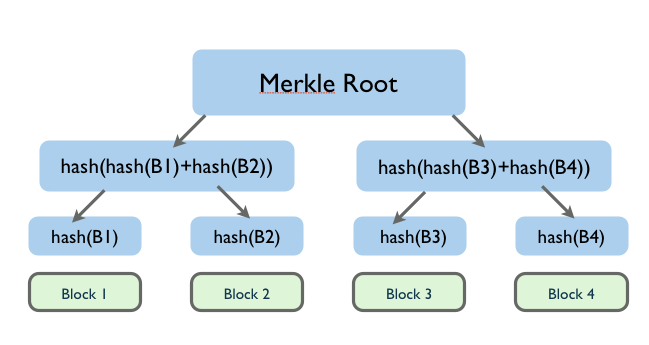
\includegraphics[width=\textwidth,keepaspectratio]{img/blockchain-hash-tree.jpg}
                \caption{Visualisation of Merkle tree}
                \label{obr 1.1.1}
            \end{left}
        \end{minipage}
    \end{left}
\end{figure}

Satoshi Nakamoto, the creator of Bitcoin, claims to be Japanese born in April 1975. It’s unclear whether it’s male or female, single person or a group of people. His or her real identity is well-hidden secret and the main topic of many speculations \cite{satoshi}. 
In 2008, through an online domain \url{bitcoin.org}, the creator of Bitcoin released a white paper. Satoshi outlines how Bitcoin will work using computer networks. The purpose was to eliminate third-party mediators from digital transactions, because of the mediation costs and to remove a single point of failure. Creation of Bitcoin is linked to the financial crisis in 2008. Cause of the crisis were risky loans given out to the people that were unable to pay them back. Multiple banks had to file bankruptcy, and all the money that belonged to the people who trusted the financial institution were lost forever.  
Nakamoto never mentioned blockchain in his first work, he only used words \emph{block} and \emph{chain} separately. Later in 2009, Satoshi Nakamoto released a whitepaper about the technology. In the whitepaper, he described how the technology was well equipped to enhance digital trust given the decentralization aspect that meant nobody would ever be in control of anything. 
\section{Cryptocurrency}
Cryptocurrency is a digital currency in which encryption techniques are used to control the generation of units of currency and verify the transfer of funds, operating independently of one single central unit  \cite{fintech_compendium}. Cryptocurrencies use decentralized control instead of a single authority like a bank. Decentralization is achieved by using distributed ledger technology - a block chain that publicly stores all transactions in it. 

In the case of centralized banking, the supply of currency is in charge of government institutions like the European Central bank. This way the value of a currency can be adjusted by adding or removing money from circulation. This is not possible with decentralized cryptocurrency where governments or corporations can't produce new units. Cryptocurrencies are by design gradually decreasing the production of their currency with predetermined market cap - the maximum amount of currency that will be in circulation. 

We need to distinguish electronic money from digital currency. 
\begin{description}
\item[Electronic money]
we currently have in our bank account can be considered an electronic version of the cash we would otherwise have in our wallets. Whenever a user uses his electronic money to pay for a service online it's the equivalent of paying in cash. \item[Digital currency]  (or virtual) currency is an electronically issued currency the transferability of which into  fiat currency is not guaranteed by the state. Digital currency can be divided into centralized and decentralized. The best example of centralized digital currency is World Of Warcraft Gold  - the currency used in a computer game.
\end{description}

\subsection{Bitcoin}
Currently the world's most used and most valued digital currency. Cryptocurrencies like Bitcoin dramatically fluctuate in value. In its peak Bitcoin was worth almost \$20000. During its peak Bitcoin was really popular among regular people, the media were talking about it, especially in the period of December-January 2018 as we can see in the graphs below.

\begin{figure}[H]
    \begin{left}
        \begin{minipage}{\linewidth}
            \begin{left}
                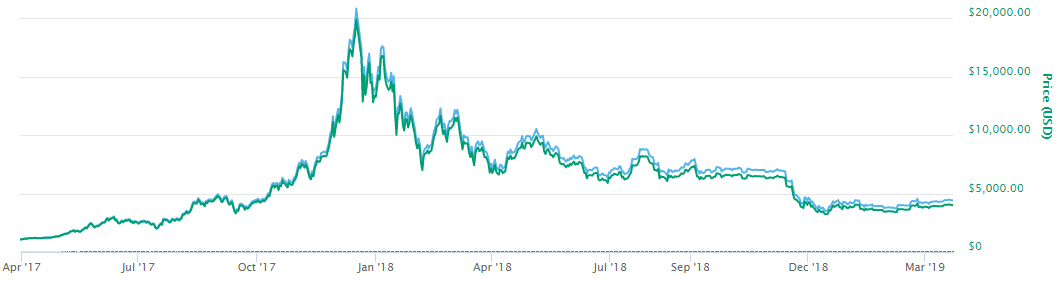
\includegraphics[width=\textwidth,keepaspectratio]{img/bitcoin_value.png}
                \caption{Bitcoin Value from April 2017 to March 2019}
                \label{obr 1.2.1}
            \end{left}
        \end{minipage}
    \end{left}
\end{figure}

\begin{figure}[H]
    \begin{left}
        \begin{minipage}{\linewidth}
            \begin{left}
                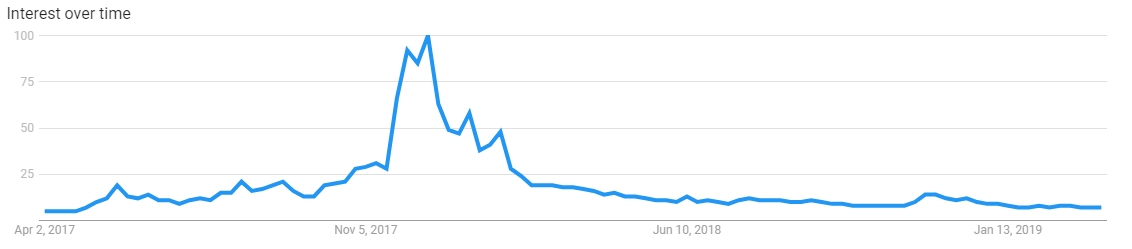
\includegraphics[width=\textwidth,keepaspectratio]{img/bitcoin_trends.png}
                \caption{Bitcoin Google search trends from April 2017 to March 2019}
                \label{obr 1.2.2}
            \end{left}
        \end{minipage}
    \end{left}
\end{figure}

Sending Bitcoin from one owner to another is called a transaction. The transaction has to be broadcasted to every peer in the network so they can update their copy of blockchain. After a broadcast was received, the network has to agree who has the latest version of blockchain with the new transaction. A node that has added a new block to the block chain is rewarded with a specific amount of Bitcoin. This process is called mining and it's the only way that new Bitcoins are created. The reward is getting smaller and will reach zero when the circulating supply of Bitcoins will be 21,000,000 BTC \cite{coinmarketcap_btc}. That reward started at 50 bitcoins per block. Every four years the protocol is adjusted, reducing the reward by half. One day the reward will be very small, but miners can also be rewarded by collecting fees volunteered by users that request transactions. This process takes around 10 minutes and it's called mining. A more detailed description of mining is available in section \hyperref[timestamping]{\textit{Time-Stamping schemes}}. 

\subsection{Etherium}
Ethereum was proposed in late 2013 and deployed in 2015 by Vitalik Buterin, a cryptocurrency researcher and programmer. It is an open blockchain platform that lets anyone build and use decentralised applications that run on blockchain technology. Like Bitcoin, no one controls or owns Ethereum – it is an open-source project \cite{eth_docs}.
The value of the Ethereum currency called Ether grew over 13 000\% in 2017, to over \$1400 and has fallen to \$130\cite{coinmarketcap}. Ether is the cryptocurrency that actually is the fuel, often referred to as a gas of this blockchain based platform. 
Ether is different from Bitcoin in several aspects. Time to add blocks to the blockchain is reduced from 10 minutes to 14-15 seconds. It uses the Ethash algorithm which reduces the advantage of specialized ASIC in mining. Transaction fees differ by computational complexity, bandwidth use and storage needs (in a system known as gas), while bitcoin transactions compete by means of transaction size, in bytes. Ethereum gas units each have a price that can be specified in a transaction. This is typically measured in Gwei. Bitcoin transactions usually have fees specified in satoshis per byte. Transaction fees are generally considerably lower for ether than for Bitcoin. In December 2017, the median transaction fee for ether corresponded to \$0.33, while for Bitcoin it corresponded to \$23. 

\subsection{Other}
CoinMarketCap lists more than 2000 cryptocurrencies while United Nations legal tender recognizes 180 currencies used worldwide \cite{List_of_circulating_currencies}. Other currencies are usually forked from Bitcoin Core, often referred to as AltCoins. AltCoin is an abbreviation of “Bitcoin alternative,” and  describes every single cryptocurrency except for Bitcoin. Altcoins are referred to as Bitcoin alternatives because, at least to some extent, most altcoins hope to either replace or improve upon at least one Bitcoin component. \cite{altcoin}. One of the signs of over saturation of the crypto market is the existence of parody coins like Dogecoin which was created as a joke currency. 

\subsection{Criticism}
Being decentralized and anonymous network open to everyone in the world, cryptocurrency faced criticism because of the lack of regulations, illegal activity and money laundering.

One of the early adopters of cryptocurrency were illegal markets as SilkRoad which accepted payments exclusively using Bitcoin. Estimated  turnover on the Silk Road anonymous online marketplace, the first to  support  Bitcoin  transactions  exclusively,  reached  \$15  million  per  year  just  one  year after it began operation. Any user holding bitcoins faces market risk via fluctuation in the exchange rate between bitcoin and other currencies. \cite{bitocin_doi}

A new type of malicious code became suddenly has become more and more popular. During one day ransomware WannaCry encrypted data on at least 75,000 computers in 99 countries. WannaCry encrypted all user data and demanded a ransom that could be only paid using  to decrypt the data. Russia's interior ministry, computers, hospitals in the United Kingdom, Telefonica in Spain, many schools in China were affected by this ransomware. The attack left hospitals and doctors unable to access patient data and led to the cancellation of operations and medical appointments. \cite{ransomware} 

Bitwise, a crypto-asset management firm, analyzed 81 exchanges, finding that 71 of them exhibited patterns that reflected artificial trading volume. One way to manufacture volume is via a technique called wash trading, in which someone simultaneously buys and sells the same asset. Although the exchanges in the study reported a combined \$6 billion in daily volume during four days this month, Bitwise determined that only \$273 million of it was real. \cite{bitwise_bitwise}
\section{Private-Public blockchain}
Publicly available software that ordinary people use every day is only a small fraction of all software. A lot of software and data is hidden behind corporate walls. Not every piece of information should be public and some of them are very sensitive. Companies often use software exclusively in their private networks to prevent unwanted data leaks or to protect themselves. Blockchain is no exception. It can be used worldwide where everyone can join the network and participate in the network as it can be used in a closed environment. Public and private blockchain share a lot of similarities. Both are decentralized P2P networks, where participants maintain a copy of a shared, synced append-only ledger of digitally signed transactions promising a guarantee if immutable data even when some participants are faulty or malicious. The main distinction between private and public is about who is allowed to participate in the network.
\begin{description}

\item[Public blockchain] is open to everyone willing to join. Even though everyone can join, participants in the network are completely anonymous. Everyone can download the whole blockchain and read the data. Currently the largest operational public blockchain network is the one behind Bitcoin. As of 2019, the current size of Bitcoin blockchain is more than 222 GB \cite{blockchain_size}. 

Public blockchains like Bitcoin consume an enormous amount of energy, time and money because of the mining and hence in return ensure trustlessness and remain tamper resistant. Bitcoin's current estimated annual electricity consumption is almost 50 TWh. About as much as Portugal uses in a year, worth around \$2,488,567,816  \cite{Bitcoin_Energy}. 


\begin{figure}[H]
    \begin{left}
        \begin{minipage}{\linewidth}
            \begin{left}
                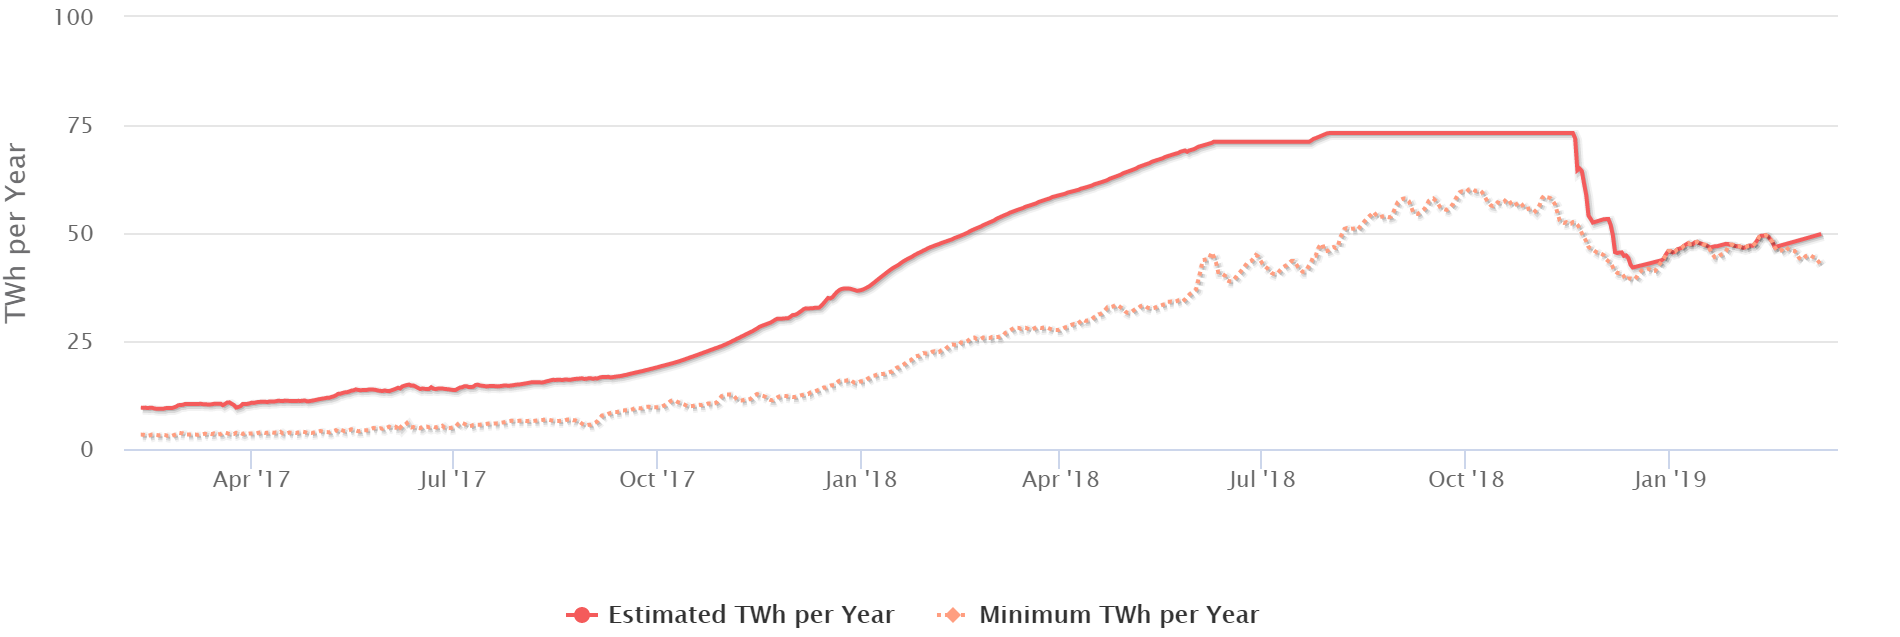
\includegraphics[width=\textwidth,keepaspectratio]{img/Bitcoin_Energy_Consumption_Index.png}
                \caption{Bitcoin Energy Consumption Index}
                \label{obr 1.3.1}
            \end{left}
        \end{minipage}
    \end{left}
\end{figure}



\item[Private blockchain] usually contains sensitive or internal information, therefore they're usually hosted in private network. Use of private blockchain is an answer to the enterprise use cases which requires performance characteristics that the permissionless blockchain technologies are unable to deliver.  

Following requirements for enterprise use of blockchain

\begin{itemize}
    \item Participants must be identified/identifiable
    \item Networks need to be permissioned
    \item High transaction throughput performance
    \item Low latency of transaction confirmation
    \item Privacy and confidentiality of transactions and data pertaining to business transactions
\end{itemize}


An invitation is required to join and new node must be validated by either the network starter or by a set of rules put in place by the network starter \cite{private_public_blockchain}. It's adding more security and transparency to help enterprises do business. Opposed to the public blockchain, private is much faster and cheaper because computers don't  have to spend an enormous amount of energy, time and money to reach a consensus. 
\end{description}

\section{Properties of blockchain}

All parties in the block chain network have the same copy of the block chain. It's in the best interest of the participant to verify it in order to receive rewards for the network. In a system where each participant owns a copy of a database, we need to prevent addition of illegitimate block. The traditional model requires a central authority which is trusted to be honest to confirm a transaction. If this point of the network is going to be compromised an attacker could cause extensive damage to the system. Blockchain solution eliminates the central authority by distributing the copies of records to the peers, they broadcast changes by forming new blocks and requesting validation based on the rules of the consensus model.  Once validated, the block is added to everyone’s chain. The process is potentially safer than the traditional model, and the middleman agent isn't required, invoking a disruption to the status quo.

\begin{figure}[H]
    \begin{center}
        \begin{minipage}{\linewidth}
            \begin{center}
                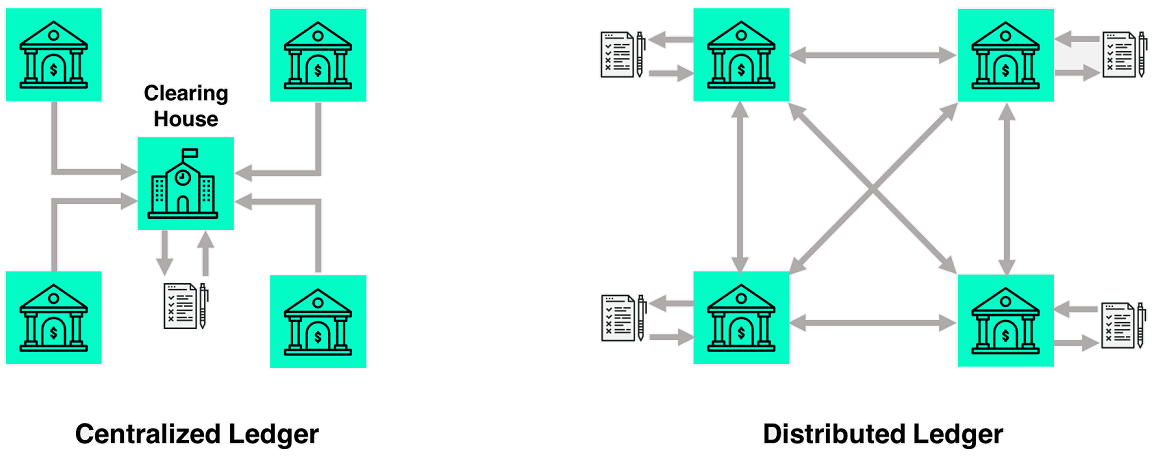
\includegraphics[width=\textwidth,keepaspectratio]{img/centralized_vs_distributed.png}
                \caption{Centralized and distributed ledger \cite{tradeix}}
                \label{obr 1.2.1}
            \end{center}
        \end{minipage}
    \end{center}
\end{figure}

Blockchain is an ongoing chain of blocks records, forming a sequential linked list with hash pointers and separately containing data. A blockchain is typically redundantly distributed across a P2P network, that verifies the integrity of existing blocks and adds new blocks to serve as a distributed database. Verification obeys a set of protocol rules, the codebase. The goal of a blockchain is to be secure by design with a tamper-proof validation of data at a time. We can summary blockchain properties into \cite{Conceptualizing}

\begin{description}
\item[Immutability] (permanent and tamper-proof)  a blockchain is a permanent record of  transactions. Once a block is added, it cannot be altered.  This creates trust in the transaction record.
\item[Security] (trust verification) each block on the blockchain is verified independently via a Consensus model which provide rules for validating a block, and often use a scarce resource (such as computing power) to show proof that adequate effort was made.  In Bitcoin, this is referred to as the mining process.  works without the use of a central authority or an explicit trust-granting agent.
\item[Decentralization] (networked copies) a blockchain is stored in a file that can be accessed and copied by any node on the network.  This creates decentralization.
\end{description}

\section{Asymmetric cryptography}

Asymmetric cryptography, also known as public-key cryptography, is one of the key components of blockchain technology. This form of cryptography allows everyone to verify the integrity of the transaction. Public Key Cryptography is a cryptographic system that relies on a pair of keys, a private key which is kept secret and a public key which is broadcasted out to the network. We can think of a public key as a user name which can be displayed on the internet without any concerns about security. On the other hand, a private key is password that tightly coupled with the user name. It's practically impossible to derive the private key from a public key. 



\begin{figure}[H]
    \begin{center}
        \begin{minipage}{\linewidth}
            \begin{center}
                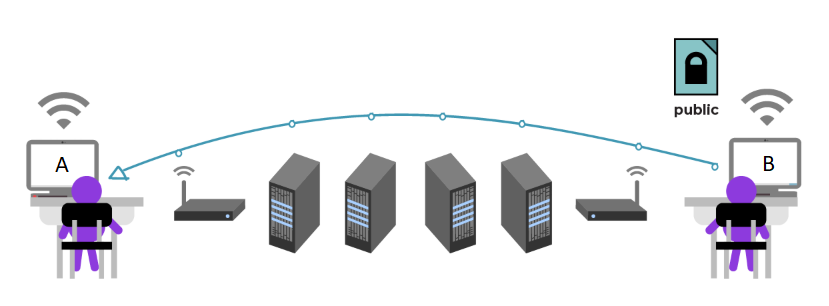
\includegraphics[width=\textwidth,keepaspectratio]{img/asymetric1.png}
                \caption{Sending encrypted message \cite{SSD.EFF.ORG}}
                \label{obr 1.2.1}
            \end{center}
        \end{minipage}
    \end{center}
\end{figure}

If person $A$ wants to send an encrypted message to $B$ to be sure that only $B$ will be able to read it without any intermediates $A$ has to use $B$'s public key to encrypt a message. This message can be send through many computers and not a single one would be able to read the content of the message. Intermediaries such as the email service providers, Internet service providers, and those on their networks—are able to see meta-data this whole time: who is sending what to whom, when, what time it’s received, what the subject line is, that the message is encrypted  \cite{SSD.EFF.ORG}.
Once the message is received by $B$, he has to use his securely stored private key to decrypt the message. 

\begin{figure}[H]
    \begin{center}
        \begin{minipage}{\linewidth}
            \begin{center}
                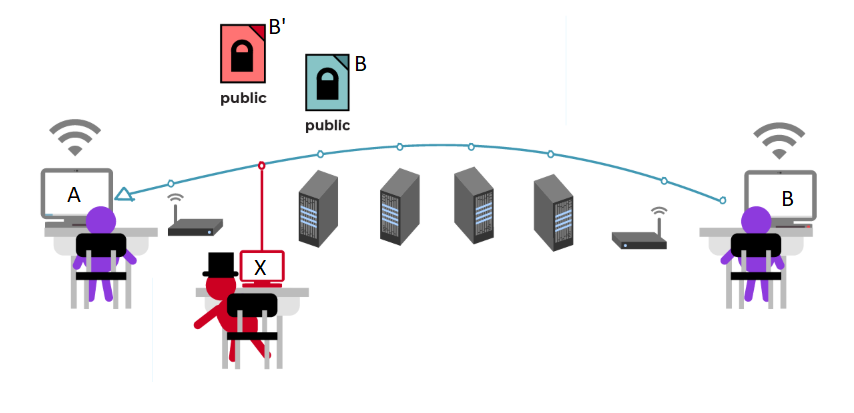
\includegraphics[width=\textwidth,keepaspectratio]{img/asymetric2.png}
                \caption{Sending encrypted message with the man in the middle \cite{SSD.EFF.ORG}}
                \label{obr 1.2.1}
            \end{center}
        \end{minipage}
    \end{center}
\end{figure}

If an intermediary with a bad intention finds a way to convince $A$ to use wrong public key $B'$ to send $B$ a message he can alter or read the message. This attack is called \emph{man in the middle attack} which consists of $X$ creating a keypair $B'$. Once the message has been captured by $X$ he can decrypt the message using his private key for $B'$, read or alter the message and encrypt it using the real $B$ public key and forward it to the recipient. 
This can be avoided by using \emph{fingerprints} or hashes of the public key. Parties that want to have a secured conversation should share their fingerprints of public keys preferably in person or through a different secured channel and verify the public key before encrypting the message.

Using private-public key encryption we can digitally sign a document to verify that the sender is legitimate. The sender $A$ with public key $KV_A$ and private key $KT_A$ signs his message $M$ such that he attaches the result of deciphering of message $M$ with his private key $KT_A$ 

\begin{center}
    $Sig(M) =D_{KTA}(M)$
\end{center}.

The receiver $B$ tests the authenticity of the signature so that he encipherers the signature with public key $KVA$ of the sender – calculates
\begin{center}
    $M'=E_{KVA(Sig(M)}$
\end{center}

and check whether $M = M'$. If $M' \neq M$, then the message was forged or the signature is not genuine. If $M' = M$, then the signature is genuine and the message is unchanged. The only person – the sender $A$ – could create $Sig(M) = D_{KTA}(M)$ for message $M$ since he is the only participant who has private key $KTA$. \cite{OneWayHashFunctions}

Major cryptocurrencies like Bitcoin and Ethereum function using three fundamental pieces of information: the address, associated with a balance and used for sending and receiving funds, and the address’ corresponding public and private keys. The generation of address begins with the generation of a private key. From there, its corresponding public key can be derived using a known algorithm. The address, which can then be used in transactions, is a shorter, representative form of the public key.

The private key is what grants a cryptocurrency user ownership of the funds on a given address. The Blockchain wallet automatically generates and stores private keys for you. When you send from a Blockchain wallet, the software signs the transaction with your private key without actually disclosing it, which indicates to the entire network that you have the authority to transfer the funds on the address you’re sending from.

The security of this system comes from the one-way street that is getting from the private key to the public address. It is not possible to derive the public key from the address; likewise, it is impossible to derive the private key from the public key. 
\section{Time-stamping schemes}
\label{timestamping}
In a distributed network, we have to ensure that the owner of the currency can not use the same units to pay different recipients. Once money has been sent an attempt to spend them again has to be rejected by the network. For electronic money, it's not a relevant problem since transactions are handled by a central authority. In a distributed world, this problem could be solved using a consensus. Blockchains use consensus systems to make sure the information in the database is always correct, without the need for a trusted third party. Consensus algorithms enable network participants to agree on the contents of the blockchain in a distributed and trustless manner. 

\subsection{Proof of work}
A proof of work is a piece of data which is difficult (costly, time-consuming) to produce, but easy for others to verify and which satisfies certain requirements. Producing a proof of work can be a random process with low probability so that a lot of trial and error is required on average before a valid proof of work is generated \cite{proof_of_work}. 

If a node wants to add a new block to the network in order for a block to be accepted by network participants, miners must complete a proof of work which covers all of the data in the block. The difficulty of this work is adjusted so as to limit the rate at which new blocks can be generated by the network to one every 10 minutes. Due to the very low probability of successful generation, this makes it unpredictable which worker computer in the network will be able to generate the next block. 

Bitcoin uses the hashcash Proof of work function which was invented in 1997 by Adam Back \cite{Hashcash}. It was used as an anti-denial of service tool preventing mass email sending. Original hashcash algorithm used SHA1 as it's hash function, but Bitcoin adopted newer SHA256. 

Each block is represented by a \emph{block hash} - hash of a block header

\begin{table}[H]
\centering
\caption{Bitcoin's block header}
\begin{tabular}{|l|l|}
\hline
\textbf{Field}      & \textbf{Description}                                                                                                                         \\ \hline
Version             & The version of the block.                                                                                                                    \\ \hline
Previous Block Hash & The Block Hash of the block that this block is being built on top of.                              \\ \hline
Merkle Root         & All of the transactions in this block, hashed together.      \\ \hline
Time                & Current unix timestamp. \\ \hline
Bits                & A shortened version of the Target.Also known as difficulty                                                                                                           \\ \hline
Nonce               & Variable field.                     \\ \hline
\end{tabular}
\end{table}

As an example of proof of work, we'll take a look at mining Bitcoin's block number 123456.

\begin{table}[H]
\caption{Bitcoin's block #123456}

\begin{tabular}{|l|l|}

\hline
\textbf{Field} & \textbf{Value}                                                   \\ \hline
version        & 0x00000001                                                       \\ \hline
previousblock  & 0000000000004df94b4488e034359e862725dc969c498b9678dc261c58a679dc \\ \hline
merkleroot     & 271bb1df11fbb9aaf1e06b7719843635e057808fd9a4daee7c30070eb8d7ad50 \\ \hline
time           & 12 May 2011, 12:43:04                                            \\ \hline
bits           & 0x\emph{1A}6A93B3                                                         \\ \hline
nonce          & Value to be mined                                                                 \\ \hline
\end{tabular}
\end{table}

We will convert bits \texttt{0x\emph{1A}6A93B3} to target  
\begin{center}
    \texttt {0x6A93B3} . $2^{8(\texttt{0x1A} - 3)}$ = \texttt{0000000000006a93b3000000000000000000...}
\end{center}

Now miner will try every possible value for \emph{nonce} until he gets hash with a value lower than the target. First miner which will find a nonce that is smaller than the target will be rewarded by the network. Miner with most computing power was able to find the correct value first, in this case \texttt{1160139541} which will result in hash \texttt{0000000000000b60bc96a44724fd72daf9b92cf8ad00510b5224c6253ac40095}  that is compared to the target. If it's smaller than target  correct nonce has been found and the block can be added to the ledger with the result hash


\subsection{Proof of stake}

Proof of Stake is a category of consensus algorithms for public blockchains that depend on a validator's economic stake in the network. In proof of work based public blockchains, the algorithm rewards participants who solve cryptographic puzzles in order to validate transactions and create new blocks. In PoS based public blockchains, a set of validators take turns proposing and voting on the next block, and the weight of each validator's vote depends on the size of its deposit (i.e. stake). Significant advantages of PoS include security, reduced risk of centralization, and energy efficiency.

In general, a proof of stake algorithm looks as follows. The blockchain keeps track of a set of validators, and anyone who holds the blockchain's base cryptocurrency (in Ethereum's case, ether) can become a validator by sending a special type of transaction that locks up their ether into a deposit. The process of creating and agreeing to new blocks is then done through a consensus algorithm that all current validators can participate in.

There are many kinds of consensus algorithms, and many ways to assign rewards to validators who participate in the consensus algorithm, so there are many "flavors" of proof of stake. From an algorithmic perspective, there are two major types: chain-based proof of stake and BFT-style proof of stake.

In chain-based proof of stake, the algorithm pseudo-randomly selects a validator during each time slot (e.g. every period of 10 seconds might be a time slot), and assigns that validator the right to create a single block, and this block must point to some previous block (normally the block at the end of the previously longest chain), and so over time most blocks converge into a single constantly growing chain.\cite{pos}

\subsection{Proof of Elapsed Time }

Proof of Elapsed Time follows a simple strategy, each participant in the blockchain network waits a random amount of time and the first participant to finish waiting gets to be leader for the new block. While the idea is simple at its core, nodes cannot be trusted to generate a random amount of time and actually wait for the generated period. PoET comes from Intel, and it relies on a special CPU instruction set called Intel Software Guard Extensions (SGX). SGX allows applications to run trusted code in a protected environment. For PoET, the trusted code is what ensures that these two requirements are satisfied. PoET is used in Hyperledger Sawtooth blockchain. \cite{poet}

\subsection{Proof of Capacity}

Proof of capacity is a consensus mechanism algorithm used in blockchains that allows the mining devices in the network to use their available hard drive space to decide the mining rights, instead of using the mining device’s computing power or the miner’s stake as in the proof of stake algorithm. Instead of repeatedly altering the numbers in the block header and repeated hashing for the solution value, POC works by storing a list of possible solutions on the mining device’s hard drive even before the mining activity commences. The larger the hard drive, the more possible solution values one can store on the hard drive, the more chances a miner has to match the required hash value from his list, resulting in more chances to win the mining reward \cite{pot1}. 

There are two components that make up the PoC, these are Plotting and the mining on the hard drive. Plotting is the first stage and this involves you creating your unique plot files.
Plotting makes use of a hashing function called Shabal. This hashing algorithm is much harder to compute than the SHA 256 variant used in the Bitcoin protocol. Miners will compute the nonce solutions using Shabal algorithm in advance and store them on the hard drive.
Each of the nonces will contain 8,192 hashes and these are bundled together into a number of pairs that are termed “scoops”. In total there will be 4,095 scoops that will each be assigned that unique number.

\begin{figure}[H]
    \begin{center}
        \begin{minipage}{\linewidth}
            \begin{center}
                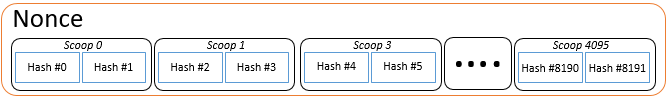
\includegraphics[width=\textwidth,keepaspectratio]{img/poc_scoops.png}
                \caption{Example of Nonce and Scoops \cite{poc}}
                \label{obr 1.2.1}
            \end{center}
        \end{minipage}
    \end{center}
\end{figure}

One of the results of the calculation will be the scoop number. This scoop number will be between 0 and 4,095. The resulting scoop number and the corresponding nonce will be used to calculate a unit of time called the “deadline”.This will be completed for all of the nonces that are on your hard drive and you will then select the shortest deadline. This minimum deadline is the amount of time that will pass since the last block was created until you can produce a new one. If the deadline that you are able to produce is shorter than those of the other miners then you are allowed to create the new block and you will be entitled to the block reward. \cite{poc}
\section{Real world use}

\subsection{e-Estonia} 
The Estonian government has been testing blockchain since 2008. Since 2012, blockchain has been in operational use in Estonia’s registries, such as national health, judicial, legislative, security and commercial code systems, with plans to extend its use to other spheres such as personal medicine, cybersecurity and data embassies.

Blockchain technology solves many of the problems that data governance professionals have been trying to solve for years. The technology developed by the Estonians is also being used by NATO, U.S. Department of Defence, as well as European Union information systems to ensure cybersecurity.

In Estonia, patients own their health data and hospitals have made this available online since 2008. Today, over 95\% of the data generated by hospitals and doctors has been digitized, and blockchain technology is used for assuring the integrity of stored electronic medical records as well as system access logs. Using blockchain technology mitigates internal threats to data, making patient’s information more secure. \cite{estionia}


\subsection{Counterfeit drug prevention and detection}

When we get sick, we trust that the doctors have our best interests at heart. We trust that the medicine we are prescribed and that we purchase will make us better instead of making our condition worse. And by and large, they do. However, that’s not always the case. Counterfeit medicine is a global problem that has adversely impacted hundreds of thousands of people across the world particularly in developing countries that do not have strong regulation structures and enforcement. According to the World Health Organization (WHO) estimates, “1 in 10 medical products circulating in low and middle-income countries is either substandard or falsified”, which ranged from flu vaccines to cancer treatment. \cite{fake_drugs}

FarmaTrust has formed a partnership with the Mongolian government to create a one-year pilot project to prevent the production and distribution of counterfeit medicines using blockchain and other emerging technologies. \cite{fake_drugs}

\subsection{Odometer fraud prevention}

The total economic costs of odometer fraud in second-hand cars traded cross-border in the European Union can be estimated to be at least €1.31 billion, with the most probable fraud rate scenario yielding €8.77 billion of economic loss. The main negative impacts of odometer fraud are borne by consumers, as their rights are breached, confidence is lowered, and maintenance and repair expenses are increased. Road safety is also impacted, as cars are not adequately maintained at the right time. \cite{odometer_fraud}

Bosch IoT Lab is developing a blockchain based solution that ensures a car’s mileage data is correct. They also published an app for consumers that enables them to view the mileage history of their car. Users can access an online service to get a digital certificate indicating whether the mileage has been manipulated or not. By using this service, consumers can easily create a digital certificate for their cars and also share the information with other entities in order to create trust in the specific car data. \cite{bosh}

\subsection{Aerospace supply chains}

Thales is a French multinational company that designs and builds electrical systems and provides services for the aerospace, defence, transportation and security markets. They faced a  problem where the Ministry of Defense had aircraft carriers that needed to be returned to the supplier because of faulty electrical systems. The issue was due to counterfeit components. It meant that the originality of the fake components had to be tracked back up a twenty tier supply chain. \cite{thales}

Aircraft are built using thousands of different suppliers, and any of these suppliers could have inserted counterfeited elements. It can cost millions of pounds to identify the origins of a counterfeit piece. Additionally, a grounded aircraft generates high revenue losses and the need to set up alternative solutions. \cite{thales}

The solution developed by Thales and Accenture uses Fabric Hyperledger allowing for easy allocation of permissions to different participants in the network.
\section{Comparison with database}

A traditional database set up is mostly a client-server type of network architecture. User with the correct log-in credentials and access permissions can query the database and make changes to it. In case of a change to the main database, every user will receive an update next time they access the database. Control of the database remains with database administrators, which allows for access and permissions being maintained by a central authority. Access to the database should be restricted by permissions so only eligible people are able to delete or update information. This works quite differently in a blockchain, in a blockchain, each participant maintains, calculates, updates and validates new entries into the database. All of the participants (nodes) work together to ensure they are all coming to the same conclusions (consensus), providing built-in security for the network. The consequences of this fundamental difference are that blockchains are well-suited as a system of record for certain functions, while a centralised database is entirely appropriate for other functions \cite{steemit}. Almost all blockchains allow different parties that do not necessarily trust each other to share information without requiring a central administrator. 

The contents of a database are stored in the memory and disk of a particular computer system, and anybody with sufficient access to that system can destroy or corrupt the data within. As a result, the moment you entrust your data to a regular database, you also become dependent on the human organisation in which that database resides. Whereas blockchain provides a database that is publicly verifiable and enabled by integrity and transparency: \cite{steemit}
\begin{itemize}
    \item Integrity because every user can be sure that the data they are retrieving is uncorrupted and unaltered since the moment it was recorded.
    \item Transparency because every user can verify how the blockchain has been appended over time.
\end{itemize}


\begin{figure}[H]
    \begin{center}
        \begin{minipage}{\linewidth}
            \begin{center}
                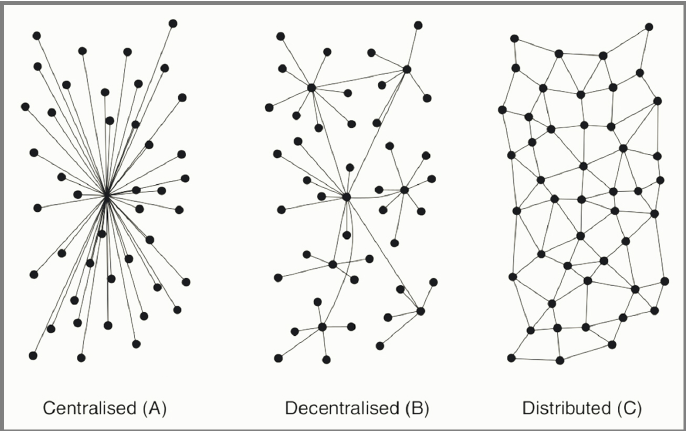
\includegraphics[width=\textwidth,keepaspectratio]{img/centralized-vs-decentralized-vs-distributed-processing.png}
                \caption{Centralized vs decentralized vs distributed processing \cite{cen_dec_dis}}
                \label{obr 1.2.1}
            \end{center}
        \end{minipage}
    \end{center}
\end{figure}

Transparency and integrity are important in elections, where you can't be sure if your vote has been counted or even if your vote was recorded into the database correctly. If an online voting system would be compromised and a person would vote for $X$ your voted could be recorded to the database as $Y$ without your knowledge. In a decentralised solution, the corrupt system would not be trusted and ignored by the network.

\begin{description}
    \item[CRUD vs Read \& Write Operations] In a traditional database, a client can perform four functions on data: Create, Read, Update, and Delete. The blockchain is designed to be append-only structure. A user can only add more data, inform of additional blocks. All previous data is permanently stored and cannot be altered. Therefore, the only operations associated with blockchains are:
    \begin{itemize}
     \item [Read Operations] this query and retrieve data from the blockchain
     \item [Write Operations] these add more data onto the blockchain
    \end{itemize}
    Every blockchain transaction must be digitally signed using a public-private cryptography scheme. This is necessary because transactions propagate between nodes in a peer-to-peer fashion, so their source cannot otherwise be proven. The generation and verification of these signatures are computationally complex and constitutes the primary bottleneck in products like ours. By contrast, in centralized databases, once a connection has been established, there is no need to individually verify every request that comes over it.

    \item[Historical vs Real-time]
    Most central databases keep information that is up-to-date at a particular moment in time, they provide more or less a snapshot of a moment in time but do not provide real-time information. Blockchain databases, on the other hand, are able to keep information that is relevant now, as well as all the information that has come before. Blockchain technology creates a database chain that has a history of itself, they grow as an ever-expanding archive of their own history while providing a real-time portrait. Thanks to their use of cryptography and Merkle trees, the historical information becomes immutable and unchangeable, the only real way to change a blockchain is to add a new transaction that offsets the previous transaction and this can only be done with the consent of all parties involved. The Ethereum hard fork was actually an instance where they reverted to an older state to cancel out a hack of the system; which may have been necessary but an undermining of the principle of blockchain. \cite{steemit2}
    
    \item[Performance] Blockchains as systems of record are considered slow as databases when compared to what is possible for digital transaction technology such as used by Visa and Paypal today. Blockchain technology requires that some speed be sacrificed. The way distributed networks are employed in blockchain technology means that they do not share and compound processing power but rather that they each independently service the network, then compare the results of their work with the rest of the network until there is a consensus that something has happened. Traditional databases, on the other hand, have been around for decades and have seen their performance increase in line with Moore's law.\cite{steemit2}
    
     \item[Robustness]
    A large benefit of blockchain-powered databases is extreme fault tolerance, which stems from their built-in redundancy. Every node processes every transaction, so no individual node is crucial to the database as a whole. Similarly, nodes connect to each other in a dense peer-to-peer fashion, so many communication links can fail before things grind to a halt. The blockchain ensures that nodes which went down can always catch up on transactions they missed. External users can send their transactions to any node, or to multiple nodes simultaneously, and these transactions propagate automatically and seamlessly to everyone else.
    This robustness transforms the economics of database availability. With regular databases, high availability is achieved through a combination of expensive infrastructure and disaster recovery. A primary database runs on high-end hardware which is monitored closely for problems, with transactions replicated to a backup system in a different physical location. If the primary database fails, activity is automatically moved over to the backup, which becomes the new primary. Once the failed system is fixed, it’s lined up to act as the new backup if and when necessary. While all this is doable, it’s expensive and notoriously difficult to get right.

\end{description}

Many of the use cases currently under discussion do not make sense. The biggest problem tends to be confidentiality. The participants in a fiercely competitive marketplace will naturally prefer the privacy of a centralized database, rather than reveal their activities to each other. This is especially true if a trusted central party already exists and can provide the neutral territory in which that database can reside. Even though there may be some cost associated with this central provider, this is more than justified by the value of the privacy retained. The only motivation for a shift to blockchains would be aggressive new regulation. Nonetheless, blockchains do have strong use cases, where disintermediation and robustness are more important than confidentiality and performance. \cite{steemit2}
 
\section{Existing platforms}

\subsection{Etherium}
Ethereum is an open blockchain platform that lets anyone build and use decentralised applications that run on blockchain technology. Like Bitcoin, no one controls or owns Ethereum – it is an open-source project \cite{eth_docs}. Ethereum was proposed in late 2013 by Vitalik Buterin, a cryptocurrency researcher and programmer. The system was deployed to production on 30 July 2015

\subsection{Hyperledger}
Hyperledger is an umbrella project of open source blockchain platforms and tools. It was founded in 2016 by Linux foundation with 30 founding members including Accenture, Fujitsu, IBM, Intel \cite{hyperledger_founding}. It was founded these can be used to build a new generation of transactional applications that establishes trust, accountability and transparency at their core while streamlining business processes and legal constraints. Hyperledger incubates handful of business blockchain technologies like distributed ledger frameworks, smart contract engines, client libraries, graphical interfaces. 

\begin{description}
\item[Hyperledger Fabric] is currently the most used private permissioned blockchain solution. It's enterprise-grade, distributed ledger based on blockchain technologies that use smart-contracts to enforce trust between parties that don't trust each other. It was introduced to provide a modular, scalable and secure foundation for industrial blockchain. 
There is a concept of “Channels” where parties that are part of a blockchain can create separate transactions privately and then pass the final state to the be recorded on the main blockchain. This is not unlike state channels in other blockchains, but there is an additional privacy layer.
All participants have known identities, maintained by what Fabric calls “Membership Service Providers” (MSP). If you’re allowing a group of 10 hospitals to participate in your blockchain, each of the 10 hospitals is known to the network. This is the key feature of Hyperledger Fabric that makes it fit well with enterprise solutions.
Consensus: Fabric doesn't use typical Proof of Work or Proof of Stake mechanisms to achieve consensus. Because it’s highly permissioned, it uses a sequence of verified transactions (based on MSP) instead. You can use chain-code to only accept a transaction if two parties who conduct a transaction both sign it and then peers that take in the transaction validate it as well. In short, all we need to worry about for now is that multiple verified participants need to sign transactions for them to get included to the ledger. This is a good fit for enterprise-based blockchains that don’t have a huge number of participants. Because the participants are known to each other, there is a natural deterrent to malicious behaviour \cite{coral_start}. 

Hyperledger Fabric also supports chaincode. Chaincode is the term for programs that run on top of the blockchain to implement the business logic of how applications interact with the ledger. Chaincode typically handles business logic agreed to by members of the network, so it may be considered as a “smart contract”. The state created by a chaincode is scoped exclusively to that chaincode and can’t be accessed directly by another chaincode. Hyperledger Fabric Chaincode APIs implementation is available in Node.js, Golang and Java. Whilst Java support was introduced recently, Node.js and Go lang APIs are quite at a mature level. 

\begin{figure}[H]
    \begin{center}
        \begin{minipage}{\linewidth}
            \begin{center}
                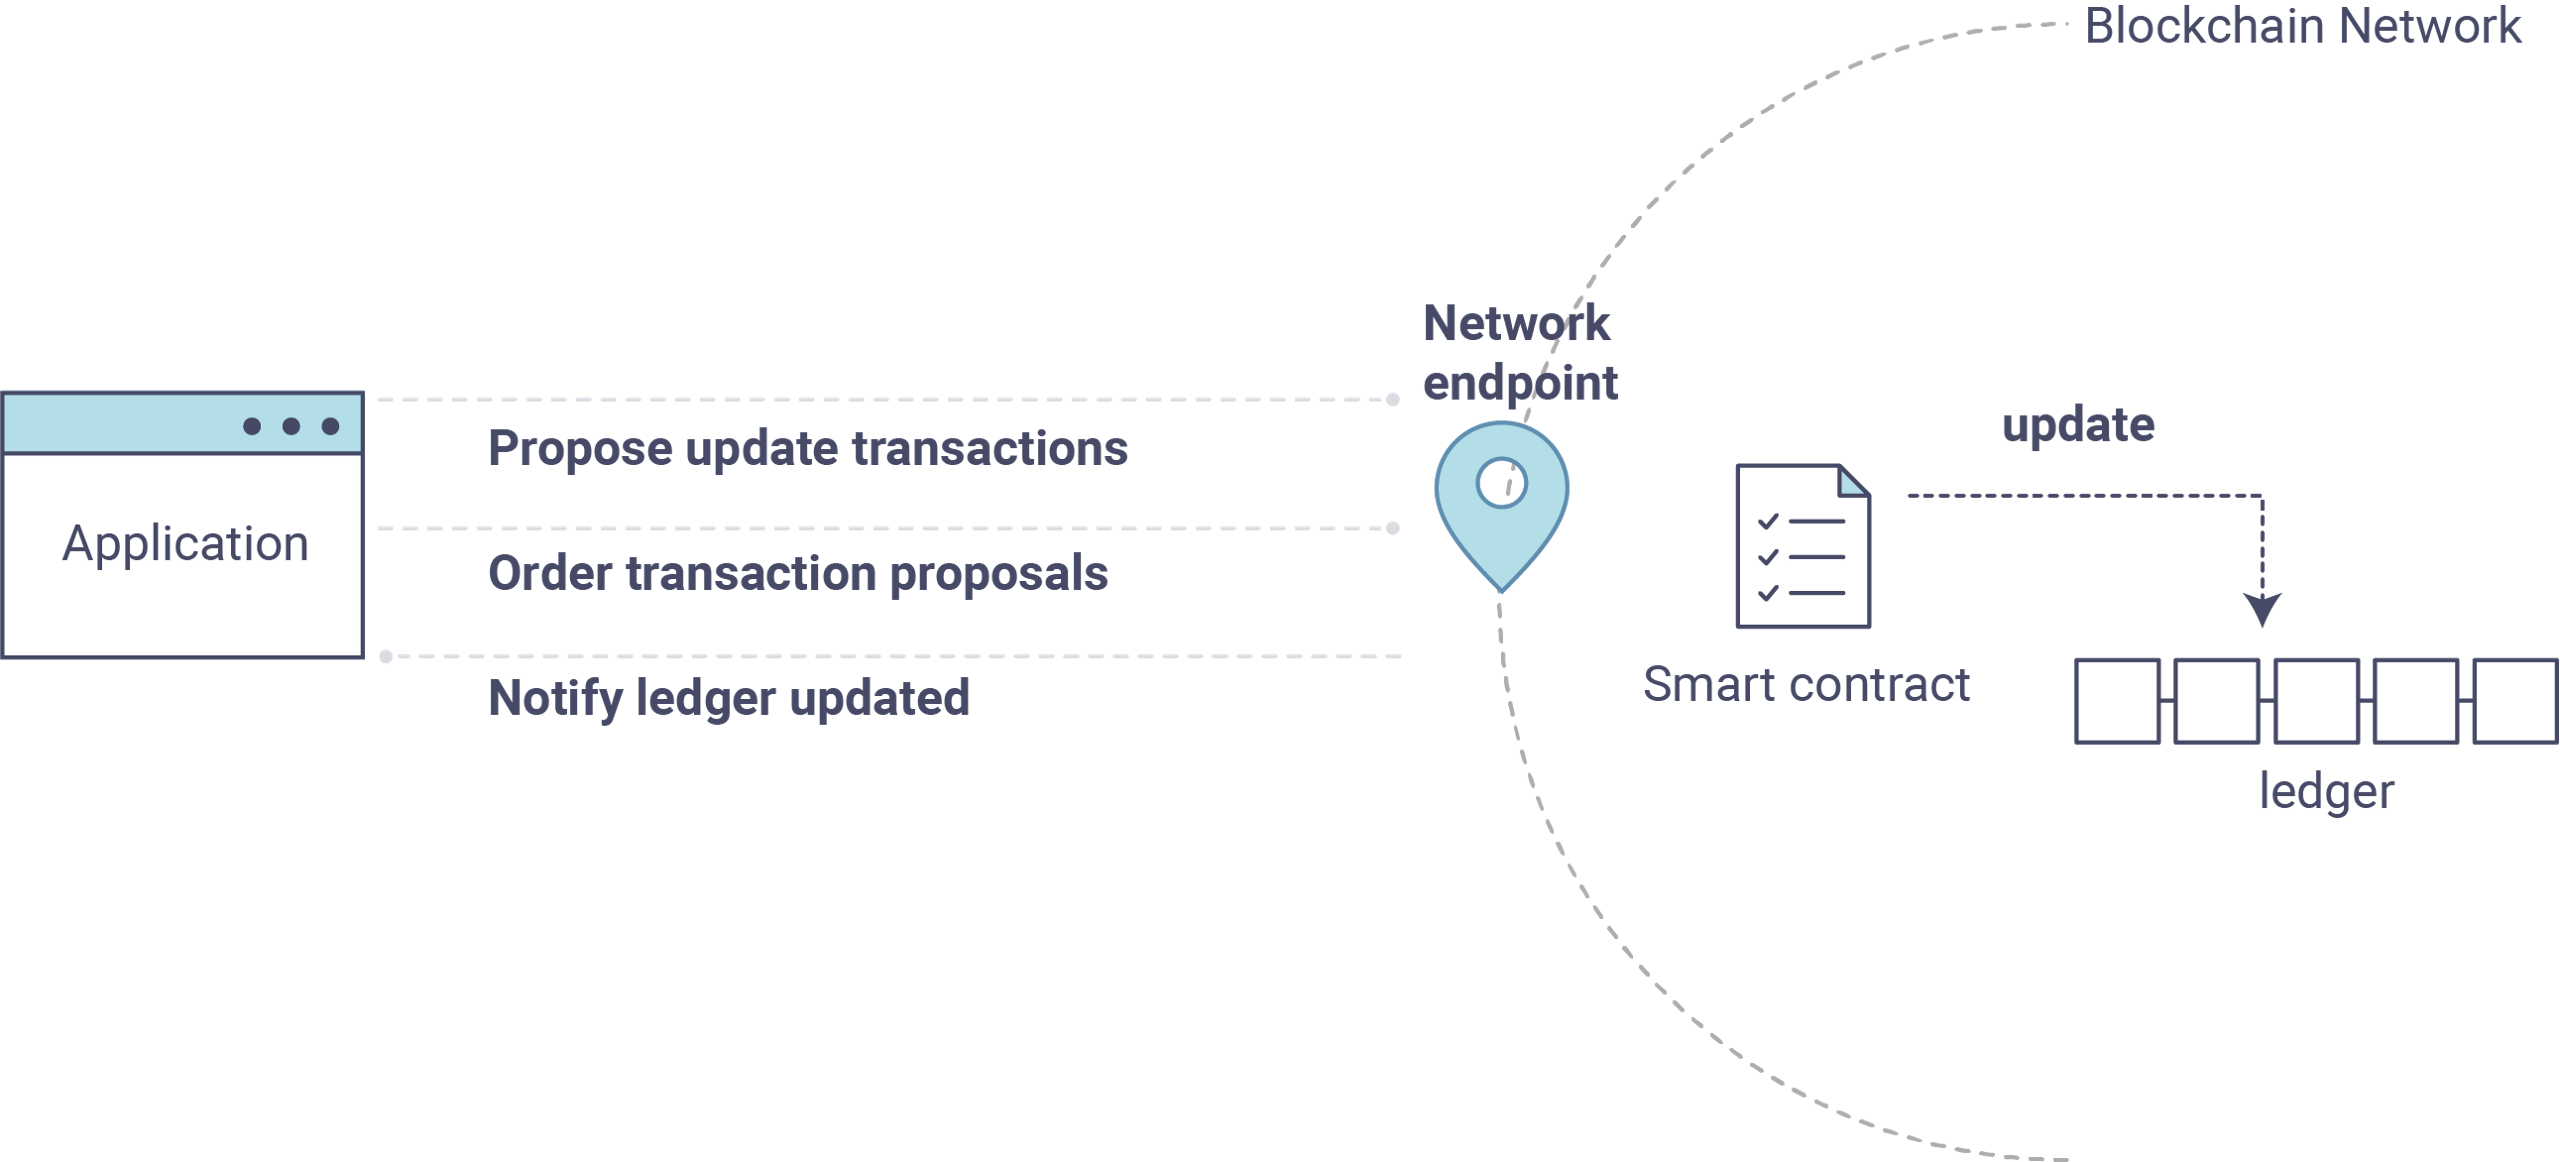
\includegraphics[width=\textwidth,keepaspectratio]{img/chaincode.png}
                \caption{Chaincode diagram}
                \label{obr 1.2.1}
            \end{center}
        \end{minipage}
    \end{center}
\end{figure}


\item[Hyperledger Sawtooth] is an enterprise blockchain platform for building distributed ledger applications and networks. Fabric and Sawtooth share a lot of common features. Main difference roots in Sawtooth support in both permissioned and permissionless blockchain implementation whereas Hyperledger Fabric support only permissioned blockchain implementation. This core difference leads to differences in the consensus algorithm. Since it's private blockchain it' doesn't make any sense to use CPU or GPU power to reach consensus, Sawtooth is using Proof of Elapsed Time (PoET). Similarly to the cryptocurrency network, peers have access to all transaction data.

\item[Hyperledger Composer] is an extensive, open development toolset and framework to make developing blockchain applications easier. The primary goal is to accelerate time to value and make it easier to integrate blockchain applications with the existing business systems. Composer can be used to rapidly develop use cases and deploy a blockchain solution. Composer allows to model business network and integrates existing systems and data with your blockchain applications. Hyperledger Composer supports the existing Hyperledger Fabric blockchain infrastructure and runtime, which supports pluggable blockchain consensus protocols to ensure that transactions are validated according to the policy by the designated business network participants. Composer is used to quickly model the current business network, containing existing assets and the transactions related to them; assets are tangible or intangible goods, services, or property. As part of the business network model we define the transactions which can interact with assets. Business networks also include the participants who interact with them, each of which can be associated with a unique identity, across multiple business networks. \cite{composer}

\item[BigchainDB] is block database with some blockchain characteristics, including decentralization, immutability and native support for assets \cite{bigchaindb}. BigchainDB consists of nodes running BigchainDB Server and related software where each node is controlled by one person or organization. BigchainDB Network is a set of BigchainDB nodes connected to each other to form a BigchainDB network. Each node in the network runs the same software. BigchainDB Consortium are people or organizations that run the nodes in a BigchainDB network belong to a BigchainDB consortium (i.e. another organization). A consortium must have some sort of governance structure to make decisions. If a BigchainDB network is run by a single company, then the “consortium” is just that company. A consortium is an organization which has a BigchainDB network, and where each node in that network has a different operator. As of 2019 BigchainDB is still not ready for production and suitable for mostly for prototyping and experimenting.

\end{description}
\section{Blockchain usage in manufacturing process}
One of the most mentioned use case for blockchain is supply chain management. It provides enhanced transparency and manufacturers can also reduce recalls by sharing logs. One of the most appealing benefits of using blockchain for data is that it allows the data to be more interoperable. Due to this, it becomes easier for companies to share information and data with manufacturers, suppliers, and vendors. Transparency in Blockchain helps reduce delays and disputes while preventing goods from getting stuck in the supply chain. As each product can be tracked in real-time, the chances of misplacements are rare. Ranging from parts suppliers, manufacturers to sellers, the automotive supply chain is a highly complex and broad sector with multiple participants. Delivering real customer value requires analysis of existing IT and business processes along with solutions that abide by the permissions of security, confidentiality, and authorization. For automotive suppliers, blockchain can be used to protect their brands from duplicate products and to create customer-centric business models. \cite{supply_chain}

\subsection{Current state}
If a big car company is not able to produce the desired product, they'll use their chain of suppliers. Supplier is required to produce a consistent and reliable product that fits requirements and is held responsible for every part he produces. 

As an example, we'll use a manufacturing of a headlight. Car company ``CarCom'' requires headlight from ``LightCom''. ``CarCom'' requires headlights with tightened screws with torque 1.5 Nm, low beam and high beam of the light has to be consistent and pass tests. Every piece has to be marked with a unique code. ``LightCom'' will have to create or buy a machine that measures and stores all this data in a database.

When ``CarCom'' receives headlights they ordered and find a defect they'll ask for manufacturing data. If ``LightCom'' doesn't provide any data ``CarCom'' can return the whole batch or never order again. Otherwise ``LightCom'' will provide all the data from the database. The company could find out that there's something wrong with the whole batch, or simply that there was one error. If ``LightCom'' finds an error they'll follow the chain of suppliers to get a refund for a broken product. Each part of the supply chain doesn't have to trust the other one. Data can be altered before sending to avoid paying for defects and blame the other part of the chain. 

\subsection{Conclusion}

Hyperledger Fabric together with Hyperledger Composer provides a foundation for more than 20 projects in production, 40 more in development \cite{showcase} and very active community. Fabric doesn't require a native cryptocurrency which eliminates useless part of the system for our use case. Fabric is also the first blockchain technology that enables the use of standard programming languages. Code on the blockchain network is asynchronous and support of language like JavaScript with its native support for asynchronous programming make it much easier and faster to develop. Fabric doesn't use PoW based consensus so no energy is wasted on computing hashes.

After experimenting with Hyperledger Fabric where I've been trying to build blockchain network from scratch multiple times for a long period of time I decided to use Hyperledger Composer for bootstrapping Fabric network. 
Hyperledger Composer makes it faster for business owners and developers to create smart contracts and blockchain applications thanks to it's modelling language. We can use Composer together with Fabric since it provides another level of abstraction and also makes it easier to join with another system thanks to exposed API.


\newpage


\vspace{10pt}


% \begin{table}[hb!]
%     \centering
%     \begin{tabular}{| l | l | }
%     \hline
%         Jazyk   &   Podiel kódu     \\  \hline
%         Java    &   46,1\%          \\  \hline
%         C       &   30,8\%          \\  \hline
%         C++     &   13,4\%          \\  \hline
%         Ostatné &   9,7\%           \\  \hline
%     \end{tabular}
%     \caption{Percentuálny podiel jazykov v AOSP}
%     \label{tab:android_code}
% \end{table}
% 
% 
% \begin{table}[H]
% \centering
% \caption{REST komunikácia}
% \label{REST komun}
% \begin{tabular}{|l|l|l|}
% \hline
% \textit{URL/Http Metóda}             & \multicolumn{1}{c|}{\textit{\textbf{GET}}} & \multicolumn{1}{c|}{\textit{\textbf{PUT}}} \\ \hline
% \textit{\textbf{uniza.sk/student}}   & Vráti kolekciu študentov                   & Nahradí kolekciu novou                     \\ \hline
% \textit{\textbf{uniza.sk/student/1}} & Zobrazí informácie o študentovi s id 1     & Nahradí staré údaje novými                 \\ \hline
% \textit{URL/Http Metóda}             & \multicolumn{1}{c|}{\textbf{POST}}         & \multicolumn{1}{c|}{\textbf{DELETE}}       \\ \hline
% \textit{\textbf{uniza.sk/student/1}} & Vytvorí novú položku a vráti jej URI       & Vymaže kolekciu                            \\ \hline
% \textit{\textbf{uniza.sk/student/1}} & Vo všeobecnosti sa nepoužíva.              & Vymaže študenta z kolekcie                 \\ \hline
% \end{tabular}
% \end{table}


\chapter{Design}

Hyperledger Fabric and Composer will be used to design and implement blockchain solution. Firstly we have to become familiar with the technologies that Fabric provides and makes it easier to develop a product. 
During the design of the blockchain network on the Windows machine, I encountered a lot of time-consuming and annoying problems that were caused by Windows itself. Since the Hyperledger project is maintained by Linux Foundation it made sense to use a Linux operating system. Unfortunately, this decision caused another problem. A lot of companies in the automotive industry use windows based systems. The Windows Control and Automation Technology developed by Beckhoff is a software system that turns almost any compatible PC into a real-time controller with a multi-PLC system is also Windows-based and a place where most of the programs are run. To overcome this issue I installed Ubuntu to VirtualBox where the solution is deployed to. This design decision also enables portability and ease of deployment.

\section{Docker}
Docker is a computer program that performs operating-system-level virtualization. Docker is used to run software packages called containers. Containers are isolated from each other and bundle their own application, tools, libraries and configuration files; they can communicate with each other through well-defined channels. All containers are run by a single operating system kernel and are thus more lightweight than virtual machine \cite{docker}. Great benefit of docker is that it can be also run within the virtual machine in VirtualBox.It's using YAML markup language to define the configuration for Docker images. Very simple syntax and ease of use make it perfect to store configurations. Docker is used by Fabric to deploy peers and nodes as containers that can be easily run.

\section{Chaincode}
To implement chaincode on Fabric network I decided to use JavaScript because of the \emph{async await} keywords which can simplify asynchronous code and make it look like synchronous code. Chaincode is supposed to be simple and implement operations that all peers agreed on. During the instantiation process, the Peer uses Docker to run a container with the chaincode inside. The Peer is responsible for managing the chaincode container’s lifecycle and networking.


\section{Hyperledger Composer}

Hyperledger Composer is a programming model containing a modelling language, and a set of APIs to quickly define and deploy business networks and applications that allow participants to send transactions that exchange assets.

%\subsection{Blockchain State Storage}
%All transactions submitted through a business network are stored on the blockchain ledger, and the current state of assets and participants are stored in the blockchain state database. The blockchain distributes the ledger and the state database across a set of peers and ensures that updates to the ledger and state database are consistent across all peers using a consensus algorithm.

%\subsection{Connection Profiles}
%Hyperledger Composer uses Connection Profiles to define the system to connect to. A connection profile is a JSON document the is part of a business network card. These profiles are usually provided by the creator of the system they refer to and should be used to create business network cards in order to be able to connect to that system.

\subsection{Assets}
Assets are tangible or intangible goods, services, or property, and are stored in registries. Assets can represent almost anything in a business network, for example, a house for sale, the sale listing, the land registry certificate for that house, and the insurance documents for that house may all be assets in one or more business networks.

Assets must have a unique identifier, timestamp and provide a way to store any data in it. To solve the issue of a frequently changed data structure of manufacturing data, I decide to provide \emph{data} field which should be used for JSON values that are already being stored in NoSQL

\subsection{Participants}

Participants are members of a business network. They may own assets and submit transactions. Participant types are modelled, and like assets, must have an identifier and can have any other properties as required.

Participants in our network will be identified as companies with an id and name. 

\subsection{Identities}
An identity is a digital certificate and private key. Identities are used to transact on a business network and must be mapped to a participant in the business network. A single identity is stored in a business network card and if that identity has been mapped to a participant, it allows the user of that business network card to transact on a business network as that participant.

Identities will consist of two customers accessing the network. Besides network admin card a user card has to be specified for every single organisation in the network.

\subsection{Business Network cards}

Business network cards are a combination of an identity, a connection profile, and metadata, the metadata optionally containing the name of the business network to connect to. Business network cards simplify the process of connecting to a business network and extend the concept of an identity outside the business network to a 'wallet' of identities, each associated with a specific business network and connection profile.

\subsection{Transactions}

Transactions are the mechanism by which participants interact with assets. This could be as simple as a participant placing a bid on an asset in an auction. What we care about in this 
Queries

Transactions in the network will represent a change of the ownership of the product. Once the product has created it should belong to the domain owner \emph{mts.sk}. As soon as the product is assembled his ownership will be transferred to the different participant on the network - to another company. After shipment of the product, the ownership should be changed to the company which has ordered the product so we can verify what state product left the manufacturer.

\section{Historian registry}
The historian is a specialised registry which records successful transactions, including the participants and identities that submitted them. The historian stores transactions as \emph{HistorianRecord} assets, which are defined in the Hyperledger. 
This asset should be used as a logging mechanism.


\section{Hyperledger Fabric Architecture}

To understand Hyperledger Fabric's architecture we have to describe underlying concepts that are part of the system.

\begin{description}

\item[Domain] is the top-level namespace for the project. Usually, the project name or the domain name is used as the Hyperledger Fabric’s domain.


\item[Orderers] exist under a domain, there are orderers who are responsible for making sure that all the peers in the network have committed a transaction. When a transaction is proposed and committed by a peer, the orderer is informed about the new transaction and it forwards and commits this block to all adjacent peers. Orderer p is responsible for consistent Ledger state across the network

\item[Certificate authorities] are responsible for handling all the access control logic, issuing the identities and permission for the users in the Hyperledger blockchain network. To connect the network every peer needs to obtain an enrollment certificate from   CA. It authorises a peer to connect to the network and to acquire transaction certificates, which are needed to submit transactions. 

\item[Peers] are nodes which are connected to clients and are responsible for committing transactions to the world state. Each peer has its own copy of transactions in a CouchDB database. An organization can have more than one peer. Though it is advised to have multiple peers in an orderer to avoid data loss, having more than 3 or 4 peers might result in higher latency rates.

\item[Organization] is a managed group of members. Each member organization in the blockchain network is responsible to setup their peers for participating in the network. All of these peers need are configured with appropriate cryptographic materials like Certificate Authority.

\end{description}

On a Hyperledger Fabric network, the flow of data for queries and transactions is initiated by a client-side application by submitting a transaction request to a peer on a channel. The initial flow of data across the network is common to both queries and transactions. Using API available in the SDK, a client application signs and submits a transaction proposal to the appropriate endorsing peers on the specified channel. This initial transaction proposal is a request for endorsement. Each peer on the channel verifies the identity and authority of the submitting client, and (if valid) runs the specified chaincode against the supplied inputs. Based on the transaction results and the endorsement policy for the invoked chaincode, each peer returns a signed YES or NO response to the application. Each signed YES response is an endorsement of the transaction.
At this point in the transaction flow, the process diverges for queries and transactions. If the proposal called a query function in the chaincode, the application returns the data to the client. If the proposal called a function in the chaincode to update the ledger, the application continues with the following steps: The application forwards the transaction, which includes the read/write set and endorsements, to the ordering service. The transaction is then relayed to the ordering service. All channel peers validate each transaction in the block by applying the chaincode-specific Validation Policy and running a Concurrency Control Version Check.
Any transactions that fails the validation process are marked as invalid in the block, and the block is appended to the channel's ledger \cite{transaction_flow}. All valid transactions update the state database accordingly with the modified key/value pairs.

\begin{figure}[H]
    \begin{center}
        \begin{minipage}{\linewidth}
            \begin{center}
                \shadowimage[width=(\textwidth),keepaspectratio]{img/transaction_flow.png}
                \caption{Fabric transaction flow }
                \label{obr 1.2.1}
            \end{center}
        \end{minipage}
    \end{center}
\end{figure}

For the purpose of re-use of our blockchain network for multiple projects, I decided for following naming and topology. Domain should always be the name of the company under which this network has been developed. Organisations will start with generic name \emph{org} because we don't know which companies will be willing to join this network. Each organisation in the consortium will have its own certificate authority and two peers to create trust in the network. Since data is the property of customer using the service we will have more instances of the network. 

\newpage
\begin{itemize}
  \item \textbf{Domain} mts.sk
  \item \textbf{Orderer} orderer.mts.sk
  \item \emph{Organizations}
  \begin{itemize}
    \item org1
    \begin{itemize}
      \item certificate authority
      \item{ peer0 $\leftrightarrow$ CouchDB state database}
      \item{ peer1 $\leftrightarrow$ CouchDB state database}
    \end{itemize}
     \item org2
    \begin{itemize}
      \item certificate authority
      \item{ peer0 $\leftrightarrow$ CouchDB state database}
      \item{ peer1 $\leftrightarrow$ CouchDB state database}
    \end{itemize}
  \end{itemize}
\end{itemize}



\begin{figure}[H]
    \begin{center}
        \begin{minipage}{\linewidth}
            \begin{center}
                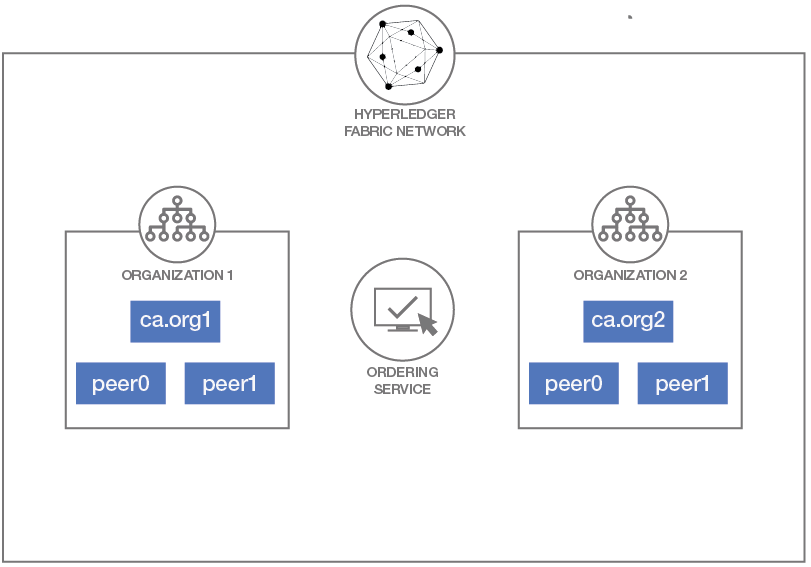
\includegraphics[width=(\textwidth),keepaspectratio]{img/my_org.png}
                \caption{Application topology}
                \label{obr 1.2.1}
            \end{center}
        \end{minipage}
    \end{center}
\end{figure}
\newpage


\chapter{Implementation}


At the beginning of the implementation I used the data model for abstract part that can be produced on any machine. Using Hyperledger Composer Modelling Language I defined assets, queries and participants. 
Since the model is very straightforward it was easy to describe it. Code is self explanatory.

\begin{figure}[H]
    \begin{center}
        \begin{minipage}{\linewidth}
            \begin{center}
                \shadowimage[width=(\textwidth),keepaspectratio]{img/code_assets.png}
                \caption{Asset code}
                \label{obr 1.2.1}
            \end{center}
        \end{minipage}
    \end{center}
\end{figure}

Chain code is installed on every peer and is responsible for executing transactions. Our transaction logic is simple and only thing that peers have to agree on is change of the product owner. Input variable \inlinecode{trade} contains new owner and product. Very important aspect of the chaincode is \inlinecode{@transaction} and \inlinecode{param} pragmas which are used to distinguish transaction code. This code is also emitting an event about the transaction so we can subscribe to the events in future.  

\begin{figure}[H]
    \begin{center}
        \begin{minipage}{\linewidth}
            \begin{center}
                \shadowimage[width=(\textwidth),keepaspectratio]{img/code_trade.png}
                \caption{Transaction code}
                \label{obr 1.2.1}
            \end{center}
        \end{minipage}
    \end{center}
\end{figure}


Thanks to Composer I was able to quickly model and deploy configuration of the network which took considerable amount of time compared to pure Fabric. To deploy blockchain network we have to firtly define high level definition of our topology. Fabric standards use \inlinecode{crypto-config.yaml} file to define system. Creating single user in this definition means to create one more user that is not an admin. Increasing number of peers would lead to generation of more peers but also higher performance demands which I wanted to avoid, especially when using virtual machine and not so powerful hardware.


\begin{figure}[H]
    \begin{center}
        \begin{minipage}{\linewidth}
            \begin{center}
                \shadowimage[width=(\textwidth),keepaspectratio]{img/code_crypto_config.png}
                \caption{Crypto-config definition}
                \label{obr 1.2.1}
            \end{center}
        \end{minipage}
    \end{center}
\end{figure}

This YAML file is then provided as an input paramater to Fabric's  \inlinecode{cryptogen} tool for generating Hyperledger Fabric key material. Cryptogen will generate all the certificates for peers and other network components

\begin{figure}[H]
    \begin{center}
        \begin{minipage}{\linewidth}
            \begin{center}
                \shadowimage[width=(0.5\textwidth),keepaspectratio]{img/crypt-gen-folder.png}
                \caption{Structure of crypto-gen}
                \label{obr 1.2.1}
            \end{center}
        \end{minipage}
    \end{center}
\end{figure}

All of the network components are secured using Transport Layer Security to encrypt communications. Certificate Authority has to create certificates for all of the network components in order to connect to those network components. The CA certificates can be found in the directory \inlinecode{crypto-config} with suffix \inlinecode{ca.crt}.

YAML file above describes topology of the network. Connection profiles with necessary certificates and addresses for connection to network components are described in \inlinecode{byfn-network.json}. This file is very important because it contains every certificate that I have generated using CA to encrypt communication over network. To avoid mistakes I copied corresponding certificates and private keys to a temporary folder for every organization and carefully defined certificates for specific peers and CA. 

\section{Deployment}

Business network card is created using \inlinecode{composer card create} command with specified connection profile for the organisation and certificates. Network card is an archive which contains connection details and certificates. Since we have two organisations \emph{org1} and \emph{org2} I created two different cards for the administrator to use to deploy the blockchain business network to the Hyperledger Fabric network.
These cards are further used to install the business network onto Fabric. 
Using this command I install business network on peers within \emph{org1}. Analogically on \emph{org2}
\begin{lstlisting}
composer network install --card PeerAdmin@byfn-network-org1 --archiveFile vortex-network.bna
\end{lstlisting}

After deployment of administrator on network we can proceed and create cards for customer access. I created cards  \emph{customera} for \emph{org1} and \emph{customerb} for \emph{org2}. 
\begin{lstlisting}
composer card create -p ./tmp/composer/org1/byfn-network-org1.json -u customera -n vortex-network -c customera/admin-pub.pem -k customera/admin-priv.pem
composer card import -f customera@vortex-network.card
\end{lstlisting}

Now we can use this business network card to interact with the blockchain business network and onboard other participants in your organization. Every operation on the network has to identified. To invoke chaincode or interact with the network the network card has to be specified as a paramater of every command. 

To avoid writing long commands I used Composer REST server to interact with the network. Hyperledger Composer includes a standalone Node.js process that exposes a business network as a REST API. The LoopBack framework is used to generate an Open API, described by a Swagger document. Following command will start a server listening at port 3000 for \emph{customerb} to interact with the network. 

\begin{lstlisting}
composer-rest-server -c customerb@vortex-network -n never -u true -w true
\end{lstlisting}

If everything works, after entering \inlinecode{localhost:3000} into our browser we should be able to see web interface generated for us.

\begin{figure}[H]
    \begin{center}
        \begin{minipage}{\linewidth}
            \begin{center}
                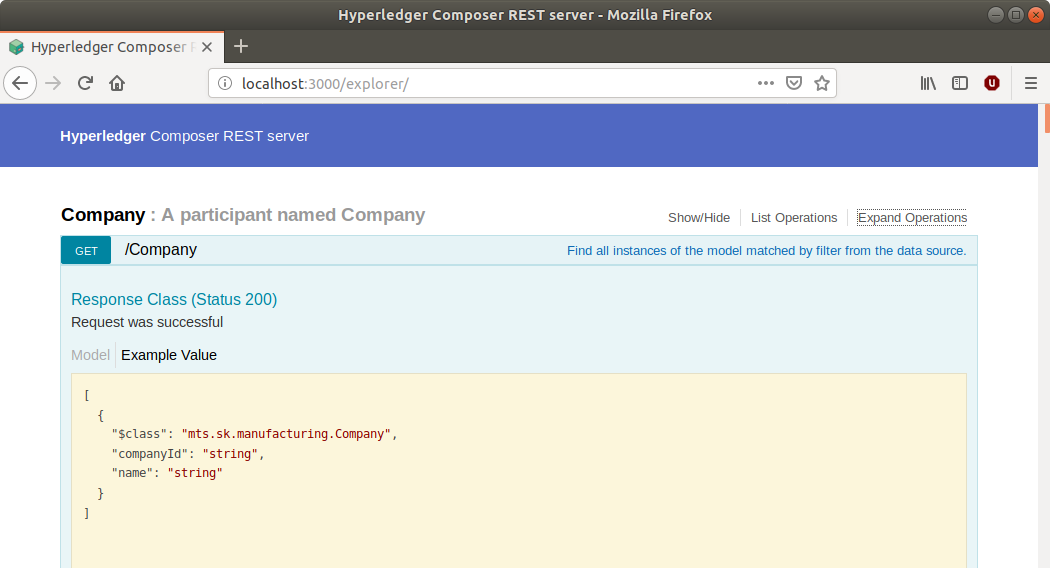
\includegraphics[width=(\textwidth),keepaspectratio]{img/composer_server.png}
                \caption{Hyperledger Composer REST server}
                \label{obr 1.2.1}
            \end{center}
        \end{minipage}
    \end{center}
\end{figure}

Having a running REST API for our blockchain network now means that we can make simple HTTP requests to the server from any application using almost every programming language we want. Generated API consists of  \emph{GET}, \emph{POST}, \emph{PUT}, \emph{HEAD} operations for managing Products, Companies, Trades and network logs. These operations follow REST standarts. 
                
When accessing blockchain network through API due to the level of abstraction it provides, it may appear to the user as a regular database. To see concrete blocks of the blockchain I wrote a simple application that uses \emph{composer-client native API} to read data in blockchain. It's simple application written in NodeJS using Express.JS framework to quickly write and deploy REST server. This application is connecting through native API and \emph{vortex-channel} to the network. 

This application is listening on port \emph{3001} and URLs described bellow.

\begin{table}[H]
\centering
\caption{ExpressJS application endpoint}
\begin{tabular}{|l|l|}
\hline
\textbf{URL}       & \textbf{Description}                                                                                                                         \\ \hline
\emph{GET} \textbackslash{blocks}\textbackslash{:id}             & Block {id} data                                                                                              \\ \hline
\emph{GET}  \textbackslash{queryInfo}\textbackslash             & Data about block height, current and previous hash data   \\ \hline

\end{tabular}
\end{table}

When accessing the blocks through \emph{blocks} interaface we can see data about the current specified block as JSON response. 

\begin{lstlisting}
  "header": {
    "number": "13",
    "previous_hash": "f6c3076842836a3fbc5f5306f73ac214804586ed5df18b3acea55383c1afcfea",
    "data_hash": "f4b1a0b59aa4d2469beed703b90921b326a1a575ab730bd8de942f7914a04a35"
  },
  "data": {
    "data": [
      {
        "signature": {
          "type": "Buffer",
          "data": [
            48,
            68,
            ...
            ]
\end{lstlisting}

Block data stores data in byte arrays and displays certificates of all nodes that were involed. When we query previous block in the chain, the \emph{previous   hash} would not match the data hash. That's beacuse a block hash is calculated by hashing over the concatenated ASN.1 encoded bytes of: the block number, previous block hash, and current block data hash.

Queryinfo endpoint queries for various useful information on the state of the Channel like height and known peers.  

Since the network is deployed in virtual machine I needed a way to connect to the REST server from hosting operating system. To achieve this connection I used \emph{Nginx} and defined a proxy pass on the port 80.

\begin{lstlisting}
server {
	listen 80 default_server;
	listen [::]:80 default_server;
	server_name _;
	location / {
		proxy_pass http://127.0.0.1:3000;
	}
	location /blocks/ {
		proxy_pass http://127.0.0.1:3001/;
}
\end{lstlisting}

This configuration takes care of requests made to the computer using http port 80  and forwards them to the application running on specific port on the local computer. Virtual machine IP address has to be in the same sub-net as is the application making requests to the server.

\section{Integration with manufacturing software}

Company MTS is using Beckhoff's PLCs with TwinCAT and develops its own software solution called \emph{Vortex} which allows easy integration with PLC code and development of complex software solutions which can satisfy costumer needs. Proprietary human machine interface (HMI) is replaced with widely used WPF and allows to use .NET framework with C\#. Modular architecture of this solution allowed easy integration of new data persistence. 

When a new product is assembled, PLC will execute command which invokes remote procedure on the PC side. Vortex is able to read whole objects in PLC as C\# objects. Generated code contains extension functions for storing plain objects without all the meta data in database. 

\begin{figure}[H]
    \begin{center}
        \begin{minipage}{\linewidth}
            \begin{center}
                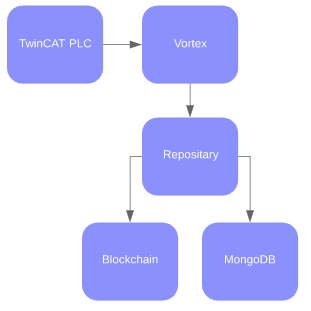
\includegraphics[width=(0.5\textwidth),keepaspectratio]{img/vortex_data.png}
                \caption{Storing data }
                \label{obr 1.2.1}
            \end{center}
        \end{minipage}
    \end{center}
\end{figure}

Interaction with database is abstracted using \emph{Repository pattern} and currently used implementation is using MongoDB because of its loose schema. 

At the same time as we are inserting new data to the database we're sending the same data as json to the blockchain. Since database implementation is in a separate project which is used by other developers only as a NuGet package, it's not their responsibility to handle storing data to blockchain. 

To communicate with REST API I used package \emph{Refit} as a type-safe REST library for .NET. To interact with the json data from the API I had to create POCO objects for the response data and define interface with endpoints as paramaters of attributes.

\begin{lstlisting}
[Get("/api/Trade/")]
Task<List<Transaction.Transaction>> GetTransactions();

[Post("/api/Trade/")]
Task<Transaction.Transaction> AddTransaction([Body] NewTransaction newtransaction);
\end{lstlisting}
\newpage

After defining singleton \inlinecode{FabricAccessor} with member\inlinecode{Fabric}

\begin{lstlisting}
 _fabric = RestService.For<IBlockchainAPI>(new HttpClient()
        {
            BaseAddress = new Uri("http://172.20.53.208/"),
            Timeout = TimeSpan.FromSeconds(5)
        });
\end{lstlisting}

Now in the repository implementation I'm able to create new Product and send it asynchronously to the blockchain with \inlinecode{data} object from the PLC.

\begin{lstlisting}
Task.Run(async () =>
    {
        var ToAdd = new Product()
        {
            ProductId = data._Id.ToString(),
            Description = "",
            Data = data.ToJson().ToString(),
            Owner = "mts.sk.manufacturing.Company#mts",
            Timestamp = data._Created.Ticks,
            Class = "mts.sk.manufacturing.Product"
        };
        await FabricAccessor.Fabric.AddProduct(ToAdd);                  
    });
\end{lstlisting}

To interact with the blockchain from the \emph{Vortex} application I followed the architecture principles of existing solution and created a new which allows user to create new companies, products, execute transactions and see the logs from the network. This small module follows principles of MVVM and uses the \inlinecode{FabricAccessor} class to get the data from API

\begin{figure}[H]
    \begin{center}
        \begin{minipage}{\linewidth}
            \begin{center}
                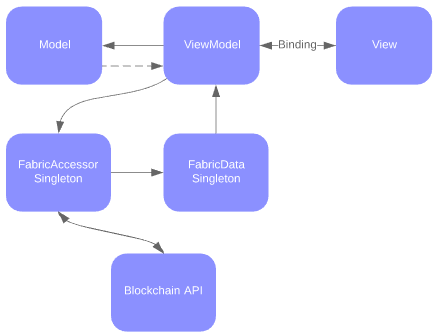
\includegraphics[width=(0.7\textwidth),keepaspectratio]{img/vortex_bc.png}
                \caption{Architecture of user module}
                \label{obr 1.2.1}
            \end{center}
        \end{minipage}
    \end{center}
\end{figure}

Data is stored in the \inlinecode{FabricDataSingleton} so if user creates a company a new object is accessible from other ViewModels immediately. This module displays necessary data for the user to interact with the ledger, displays latest transactions and logs.

\begin{figure}[H]
    \begin{center}
        \begin{minipage}{\linewidth}
            \begin{center}
                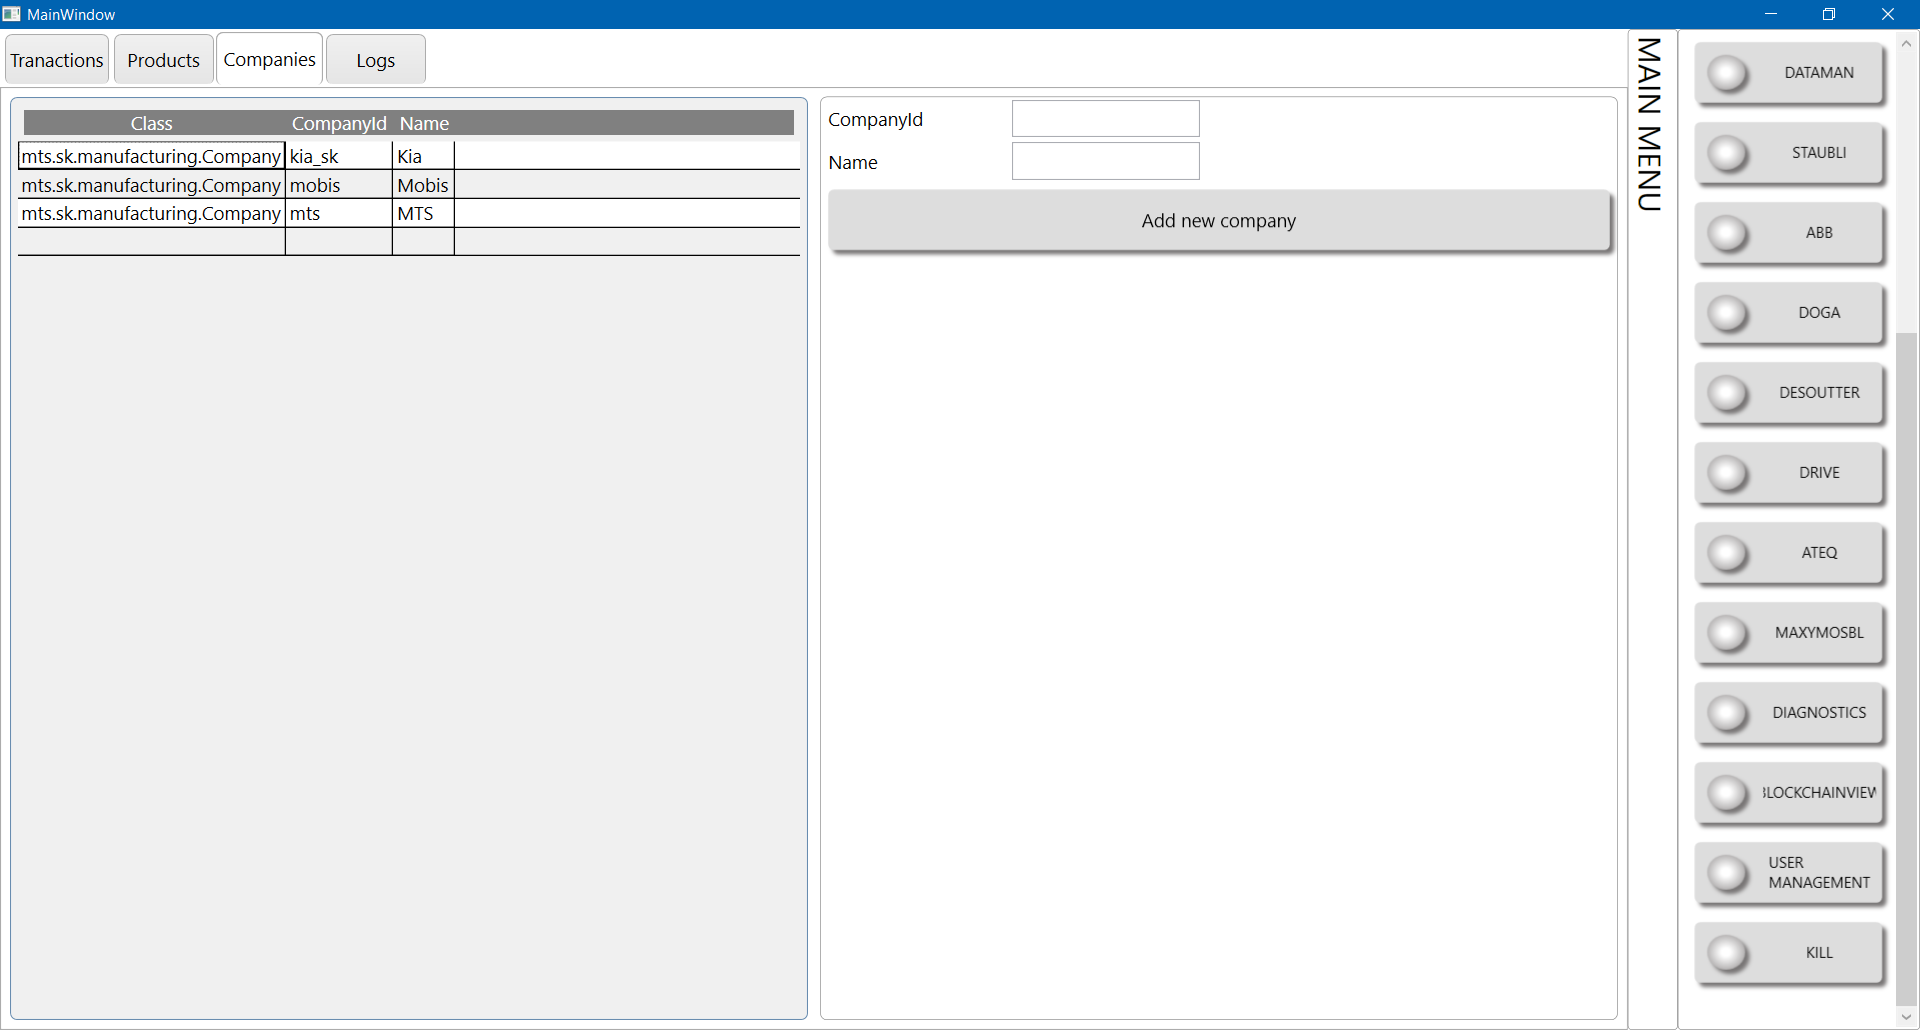
\includegraphics[width=(0.8\textwidth),keepaspectratio]{img/app/vortex_companies.png}
                \caption{Screenshot from application - companies}
                \label{obr 1.2.1}
            \end{center}
        \end{minipage}
    \end{center}
\end{figure}

\begin{figure}[H]
    \begin{center}
        \begin{minipage}{\linewidth}
            \begin{center}
                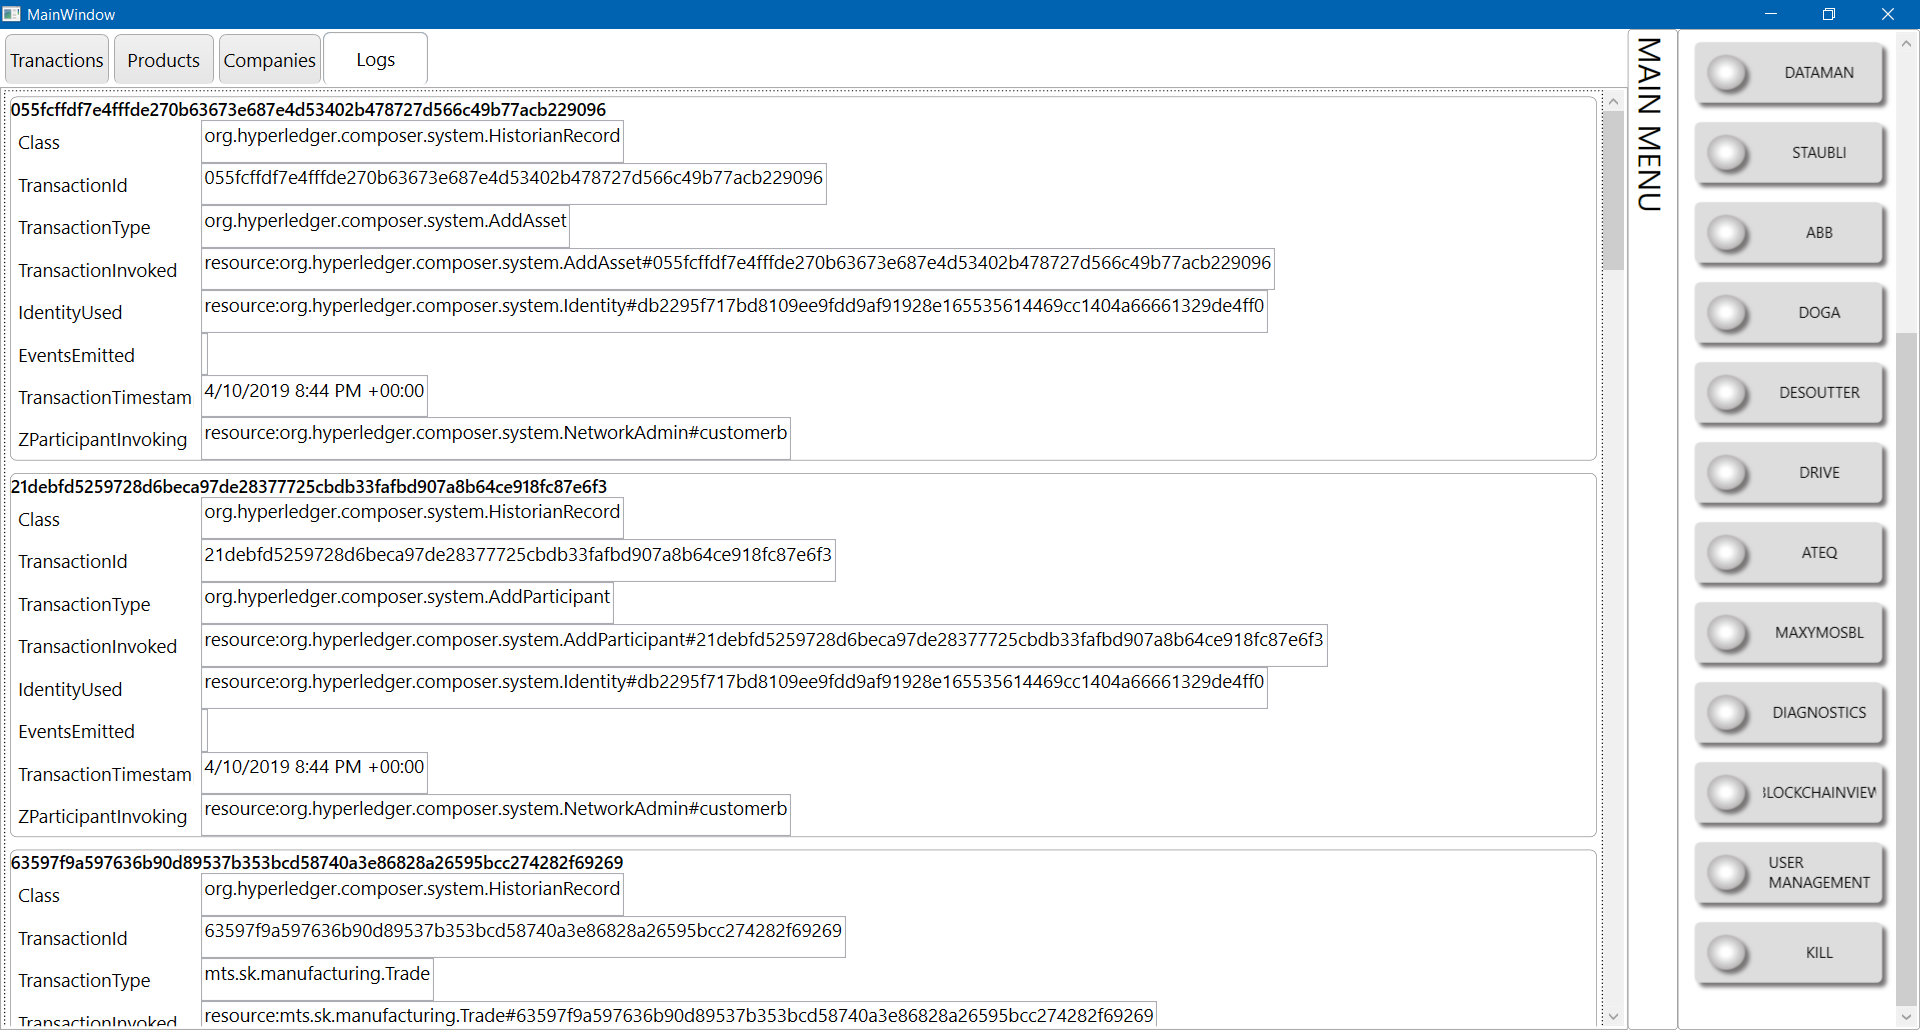
\includegraphics[width=(0.8\textwidth),keepaspectratio]{img/app/vortex_logs.png}
                \caption{Screenshot from application - logs}
                \label{obr 1.2.1}
            \end{center}
        \end{minipage}
    \end{center}
\end{figure}

\begin{figure}[H]
    \begin{center}
        \begin{minipage}{\linewidth}
            \begin{center}
                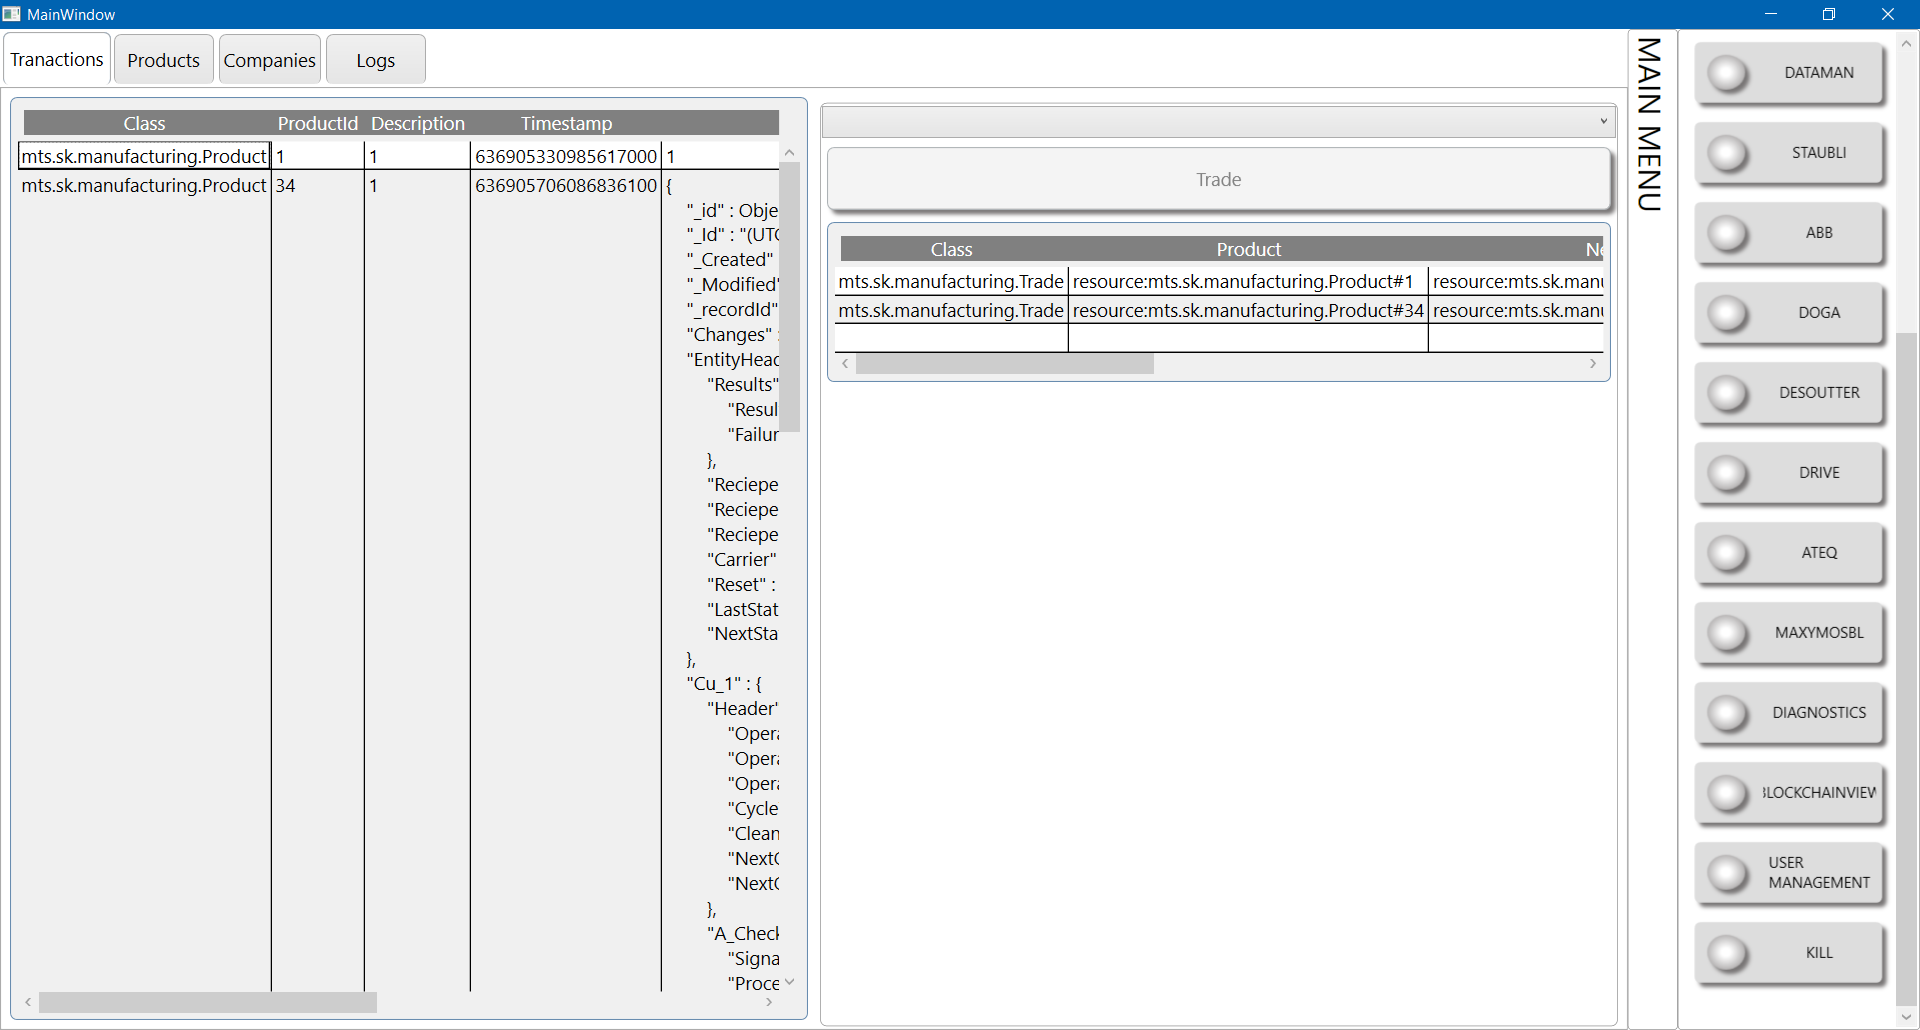
\includegraphics[width=(0.8\textwidth),keepaspectratio]{img/app/vortex_transaction.png}
                \caption{Screenshot from application - transactions}
                \label{obr 1.2.1}
            \end{center}
        \end{minipage}
    \end{center}
\end{figure}



\include{Implementation}
\chapter*{Conclusion}
\addcontentsline{toc}{chapter}{Conclusion}
In the thesis, I analyzed blockchain as a technology which originated in Bitcoin as public blockchain in the cryptocurrency world. The analysis helped to understand how public blockchains work in order to achieve consensus in decentralized systems. Best solutions for private blockchain network are covered by Hyperledger umbrella project. After experiments with Hyperledger Fabric, I concluded that it's very hard to create and maintain a working solution. Hyperledger Composer turned out to be a great tool for businesses because it saves time, therefore it saves money.  

The goal was to develop a blockchain application for storing manufacturing data which was achieved. Data is stored in a multi-organization Hyperledger Fabric business network. Storing manufacturing data to MongoDB is enriched with a blockchain without any need for another developer to modify their code in existing projects. Since this project is still in testing phase, both MongoDB and blockchain are in use, storing the same data. 

Problem with this solution is unnecessary complexity when it comes to setting up and maintenance. It might be difficult to persuade another business to pay for and implement this solution in their network. To avoid this complex solution I would recommend to reconsider the usage of blockchain. If the produced data were signed with a digital signature we could easily identify if the data has been changed in case someone has a suspicion of integrity. 

The current implementation is using Ubuntu in a virtual machine with Docker. The current version of Fabric is not very windows friendly, but with upcoming updates which may fix the issues, I encountered while using windows might be resolved. This way the future of this project will be easier deployment on windows machines. This would allow deploying peer nodes to the existing computers faster. Scripts that I wrote to simplify deployment could be used as a foundation for a configuration software which would automatically deploy peers through a network. 

Blockchain is an interesting technology providing tamper-resistant database. Mainstream adoption is questionable because current systems are complicated enough without a blockchain and it could create more problems than it solves.

%%%%%%%%%%%%%%%%%% bilbiografia

%%%%%%%%%%%%%%%%%%%%%%%%%%%%%%%%%%%%%%%%%%%%%%%%%%%%%%%%%%%%%%%%%%%%%%%%%%%%%
\begin{thebibliography}{99}                                
\label{literatura}
%\addcontentsline{toc}{section}{Literatúra}
% \addcontentsline{toc}{chapter}{Literatúra}


\bibitem{paluch_hash} 
\textit{One-Way Hash Functions} Stanislav Paluch, December [2017], online: 
\url{https://frcatel.fri.uniza.sk/users/paluch/Kryptografia/A_Krypto6.pdf}

\bibitem{wiki_hash} 
\textit{Computer Networking} CTI Reviews [2016], Cram101 Textbook Reviews ISBN: 9781467294898 

\bibitem{wiki_crypto_hash} 
\textit{Cryptographic hash function} Wikipedia, online: 
\url{https://en.wikipedia.org/wiki/Cryptographic_hash_function}

\bibitem{rainbow_table} 
\textit{Rainbow table} Learn cryptography, online: \url{https://learncryptography.com/hash-functions/rainbow-tables}

\bibitem{blockchain_history} 101Blockchains 
\textit{The History of Blockchain Technology} [November ,2018], online: 
\url{https://101blockchains.com/history-of-blockchain-timeline}

\bibitem{merkle_tree} Wikipedia
\textit{Merkle tree} , online: 
\url{https://en.wikipedia.org/wiki/Merkle_tree}

\bibitem{hyperledger_whitepaper} Hyperledger 
\textit{An Introduction to Hyperledger}, online: \url{https://www.hyperledger.org/wp-content/uploads/2018/08/HL_Whitepaper_IntroductiontoHyperledger.pdf}

\bibitem{pixel_privacy} Pixel Privacy
\textit{What is blockchain} ,online: 
\url{https://pixelprivacy.com/resources/what-is-the-blockchain/}

\bibitem{bitcoin_whitepaper} Bitcoin, \textit{ A Peer-to-Peer Electronic Cash System}, [October,2008], online: 
\url{https://bitcoin.org/bitcoin.pdf}

\bibitem{fintech_compendium} Schueffel, Patrick, \textit{ The Concise Fintech Compendium }, [2017], online: 
\url{http://www.heg-fr.ch/EN/School-of-Management/Communication-and-Events/events/Pages/EventViewer.aspx?Event=patrick-schuffel.aspx}

\bibitem{hyperledger_founding} Hyperledger, 
\textit{Linux Foundation’s Hyperledger Project Announces...}, [February ,2016],online: 
\url{https://www.hyperledger.org/announcements/2016/02/09/linux-foundations-hyperledger-project-announces-30-founding-members-and-code-proposals-to-advance-blockchain-technology}

\bibitem{intel_israel} Blockspoint, 
\textit{Blockchain Startup From Israel Receives Investments From Intel}, [October,2018], online: \url{https://blockspoint.com/news/cryptocurrency/intel-invests-in-israeli-blockchain-startup}

\bibitem{sap} Investingnews, \textit{Intel and SAP Partner} , [September ,2018], online: \url{https://investingnews.com/daily/tech-investing/blockchain-investing/intel-and-sap-partner-on-blockchain-initiative/}


\bibitem{satoshi} 101Blockchains 
\textit{Who is Satoshi Nakamoto?} [June ,2018], online: 
\url{https://101blockchains.com/who-is-satoshi-nakamoto-bitcoin}

\bibitem{eth_docs} EthDocs
\textit{What is Ethereum?} , online: 
\url{http://www.ethdocs.org/en/latest/introduction/what-is-ethereum.html}

\bibitem{blockchain_size} GetBicoin
\textit{Get Bitcoin blockchain}, online: 
\url{https://getbitcoinblockchain.com/}

\bibitem{private_public_blockchain} IBM \textit{The difference between public and private blockchain} [May,2017], online: \url{https://www.ibm.com/blogs/blockchain/2017/05/the-difference-between-public-and-private-blockchain/}


\bibitem{Conceptualizing} 
\textit{Conceptualizing blockchains: characteristics & applications }  Karim Sultan ,Umar Ruhi, Rubina Lakhan[2018], online: 
\url{https://arxiv.org/ftp/arxiv/papers/1806/1806.03693.pdf}

\bibitem{Hashcash} 
\textit{HashCash}, online: 
\url{https://en.bitcoin.it/wiki/Hashcash}



\bibitem{Bitcoin_Energy} 
\textit{digiconomist}  Bitcoin Energy Consumption Index [2019], online: 
\url{https://digiconomist.net/bitcoin-energy-consumption}


\bibitem{bitwise_bitwise} 
\textit{Nearly all Bitcoin trades are fake, apparently} MIT Technology review,online:
\url{https://www.technologyreview.com/the-download/613201/nearly-all-bitcoin-trades-are-fake-apparently/}


\bibitem{coinmarketcap}  CoinMarket Cap
\textit{Ethereum}  [March ,2019], online: 
\url{https://coinmarketcap.com/currencies/ethereum/}

\bibitem{coinmarketcap_btc}  CoinMarket Cap
\textit{Bitcoin}  [March ,2019], online: 
\url{https://coinmarketcap.com/currencies/bitcoin/}

\bibitem{coral_start} 
\textit{Coral Health} Start your own Hyperledger blockchain the Easy Way! [June ,2018], online: 
\url{https://medium.com/@mycoralhealth/start-your-own-hyperledger-blockchain-the-easy-way}

\bibitem{bigchaindb} 
\textit{BigChainDB}  Documentation [2018], online: 
\url{https://docs.bigchaindb.com/en/latest/index.html}

\bibitem{proof_of_work} 
\textit{Proof of work} bitcoin.it , online: 
\url{https://en.bitcoin.it/wiki/Proof_of_work}

\bibitem{List_of_circulating_currencies} 
\textit{List of circulating currencies} Wikipedia, online: 
\url{https://en.wikipedia.org/wiki/List_of_circulating_currencies}

\bibitem{altcoin} 
\textit{AltCoin} CCN [ ,2018], online: 
\url{https://www.ccn.com/altcoin}

\bibitem{bitocin_doi} 
\textit{Bitcoin: Economics, Technology, and Governance.} Böhme, Rainer, Nicolas Christin, Benjamin Edelman, and Tyler Moore [2015], online: 
\url{https://doi.org/10.1257\%2Fjep.29.2.213}

\bibitem{ransomware} 
\textit{Cyber-attack: Europol says it was unprecedented in scale} BBC [ ,2018], online: 
\url{https://www.bbc.com/news/world-europe-39907965}

\bibitem{composer} 
\textit{Introduction to Hyperledger Composer} online: 
\url{https://hyperledger.github.io/composer/latest/introduction/introduction.html}

\bibitem{tradeix} 
\textit{Tradeix} The Difference Between Blockchain & Distributed Ledger Technology [2018], online: 
\url{https://tradeix.com/distributed-ledger-technology/}


\bibitem{SSD.EFF.ORG} 
\textit{SSD.EFF.ORG} A Deep Dive on End-to-End Encryption [2018], online: 
\url{https://ssd.eff.org/en/module/deep-dive-end-end-encryption-how-do-public-key-encryption-systems-work}

\bibitem{OneWayHashFunctions} 
\textit{Stanislav Palúch} One-Way Hash Functions [December 2017], online: 
\url{https://frcatel.fri.uniza.sk/users/paluch/Kryptografia/A_Krypto6.pdfk}

\bibitem{pos} 
\textit{Ethereum wiki} FAQ [March ,2019], online: 
\url{https://github.com/ethereum/wiki/wiki/Proof-of-Stake-FAQ#what-is-proof-of-stake}

\bibitem{poet} 
\textit{Understanding Hyperledger Sawtooth} Kynan Rilee[February ,2018], online: 
\url{https://medium.com/kokster/understanding-hyperledger-sawtooth-proof-of-elapsed-time-e0c303577ec1}

\bibitem{pot1} 
\textit{Proof of Capacity} Investopedia [April ,2018], online: 
\url{https://www.investopedia.com/terms/p/proof-capacity-cryptocurrency.asp}


\bibitem{poc} 
\textit{Proof of Capacity Explained: The Eco-Friendly Mining Algorithm} Coinbureau [March,2018], online: 
\url{https://www.coinbureau.com/education/proof-of-capacity-explained/}

\bibitem{fake_drugs} 
\textit{Fighting Fake Drugs with Blockchain} New America , online: 
\url{https://www.newamerica.org/bretton-woods-ii/blockchain-trust-accelerator/around-the-blockchain-blog/fighting-fake-drugs-blockchain/}

\bibitem{estionia} 
\textit{e-Estionia} Homepage , online: 
\url{https://e-estonia.com/}

\bibitem{odometer_fraud} 
\textit{Odometer manipulation in motor vehiclesin the EU} Aleksandra Heflich  [January 2018], online: 
\url{http://www.europarl.europa.eu/RegData/etudes/STUD/2018/615637/EPRS_STU\%282018\%29615637_EN.pdf}

\bibitem{bosh} 
\textit{How blockchain can help to prevent odometer fraud} Bosh blog [December,2017], online: 
\url{https://blog.bosch-si.com/blockchain/how-blockchain-can-help-to-prevent-odometer-fraud/}

\bibitem{thales} 
\textit{Real-World Blockchain Implementations in Supply Chain Management} Helene Soulages [February,2018], online: 
\url{https://medium.com/blockchain-review/real-world-blockchain-implementations-in-supply-chain-management-50752b289321}

\bibitem{cen_dec_dis} 
\textit{Difference between centralized, decentralized and distributed processing} Junaid Rehman [2017], online: 
\url{http://www.itrelease.com/2017/11/difference-centralized-decentralized-distributed-processing/}

\bibitem{steemit} 
\textit{Blockchain Decrypted - Blockchain vs Database} Steemit  [2048], online: 
\url{https://steemit.com/blockchain/@iwan.spillebeen/blockchain-decrypted-blockchain-vs-database}

\bibitem{steemit2} 
\textit{Blockchains vs centralized databases}  Gideon Greenspan [2016], online: 
\url{https://www.multichain.com/blog/2016/03/blockchains-vs-centralized-databases/}

\bibitem{supply_chain} 
\textit{How is Blockchain Disrupting the Supply Chain Industry?} Mayank Pratap [August,2018], online: 
\url{https://hackernoon.com/how-is-blockchain-disrupting-the-supply-chain-industry-f3a1c599daef}


\bibitem{showcase} 
\textit{Blockchain Showcase} Hyperledger, online: 
\url{https://www.hyperledger.org/resources/blockchain-showcase}

\bibitem{docker} 
\textit{Docker} Wikipedia online: 
\url{https://en.wikipedia.org/wiki/Docker_\%28software\%29}

\bibitem{transaction_flow} 
\textit{Transaction flow} Bluemix : 
\url{https://console.bluemix.net/docs/services/blockchain/reference/v10\_fabric.html#hyperledger-fabric}



 
% Autor. Názov : podnázov (nepovinný). Poradie vydania. Miesto vydania: vydavateľ, rok vydania. Rozsah strán. ISBN

% \bibitem{cocoa_touch}
% Kelley Jeff,
% {\it Learn Cocoa Touch for iOS}, New York, Springer Science+Business Media 2012, ISBN 978-1-4302-4269-7.

\end{thebibliography}	%  Bilbiografia

\end{document}

